\documentclass{mimosis}

\usepackage{metalogo}

%%%%%%%%%%%%%%%%%%%%%%%%%%%%%%%%%%%%%%%%%%%%%%%%%%%%%%%%%%%%%%%%%%%%%%%%
% Some of my favourite personal adjustments
%%%%%%%%%%%%%%%%%%%%%%%%%%%%%%%%%%%%%%%%%%%%%%%%%%%%%%%%%%%%%%%%%%%%%%%%
%
% These are the adjustments that I consider necessary for typesetting
% a nice thesis. However, they are *not* included in the template, as
% I do not want to force you to use them.

% This ensures that I am able to typeset bold font in table while still aligning the numbers
% correctly.
\usepackage{etoolbox}

\usepackage[binary-units=true]{siunitx}
\DeclareSIUnit\px{px}

\sisetup{%
  detect-all           = true,
  detect-family        = true,
  detect-mode          = true,
  detect-shape         = true,
  detect-weight        = true,
  detect-inline-weight = math,
}

%%%%%%%%%%%%%%%%%%%%%%%%%%%%%%%%%%%%%%%%%%%%%%%%%%%%%%%%%%%%%%%%%%%%%%%%
% Hyperlinks & bookmarks
%%%%%%%%%%%%%%%%%%%%%%%%%%%%%%%%%%%%%%%%%%%%%%%%%%%%%%%%%%%%%%%%%%%%%%%%

\usepackage[%
  colorlinks = true,
  citecolor  = RoyalBlue,
  linkcolor  = RoyalBlue,
  urlcolor   = RoyalBlue,
  ]{hyperref}

\usepackage{bookmark}

%%%%%%%%%%%%%%%%%%%%%%%%%%%%%%%%%%%%%%%%%%%%%%%%%%%%%%%%%%%%%%%%%%%%%%%%
% Bibliography
%%%%%%%%%%%%%%%%%%%%%%%%%%%%%%%%%%%%%%%%%%%%%%%%%%%%%%%%%%%%%%%%%%%%%%%%
%
% I like the bibliography to be extremely plain, showing only a numeric
% identifier and citing everything in simple brackets. The first names,
% if present, will be initialized. DOIs and URLs will be preserved.

\usepackage[%
  autocite     = plain,
  backend      = bibtex,
  doi          = true,
  url          = true,
  giveninits   = true,
  hyperref     = true,
  maxbibnames  = 99,
  maxcitenames = 99,
  sortcites    = true,
  style        = numeric,
  ]{biblatex}

%%%%%%%%%%%%%%%%%%%%%%%%%%%%%%%%%%%%%%%%%%%%%%%%%%%%%%%%%%%%%%%%%%%%%%%%
% Some adjustments to make the bibliography more clean
%%%%%%%%%%%%%%%%%%%%%%%%%%%%%%%%%%%%%%%%%%%%%%%%%%%%%%%%%%%%%%%%%%%%%%%%
%
% The subsequent commands do the following:
%  - Removing the month field from the bibliography
%  - Fixing the Oxford commma
%  - Suppress the "in" for journal articles
%  - Remove the parentheses of the year in an article
%  - Delimit volume and issue of an article by a colon ":" instead of
%    a dot ""
%  - Use commas to separate the location of publishers from their name
%  - Remove the abbreviation for technical reports
%  - Display the label of bibliographic entries without brackets in the
%    bibliography
%  - Ensure that DOIs are followed by a non-breakable space
%  - Use hair spaces between initials of authors
%  - Make the font size of citations smaller
%  - Fixing ordinal numbers (1st, 2nd, 3rd, and so) on by using
%    superscripts

% Remove the month field from the bibliography. It does not serve a good
% purpose, I guess. And often, it cannot be used because the journals
% have some crazy issue policies.
\AtEveryBibitem{\clearfield{month}}
\AtEveryCitekey{\clearfield{month}}

% Fixing the Oxford comma. Not sure whether this is the proper solution.
% More information is available under [1] and [2].
%
% [1] http://tex.stackexchange.com/questions/97712/biblatex-apa-style-is-missing-a-comma-in-the-references-why
% [2] http://tex.stackexchange.com/questions/44048/use-et-al-in-biblatex-custom-style
%
\AtBeginBibliography{%
  \renewcommand*{\finalnamedelim}{%
    \ifthenelse{\value{listcount} > 2}{%
      \addcomma
      \addspace
      \bibstring{and}%
    }{%
      \addspace
      \bibstring{and}%
    }
  }
}

% Suppress "in" for journal articles. This is unnecessary in my opinion
% because the journal title is typeset in italics anyway.
\renewbibmacro{in:}{%
  \ifentrytype{article}
  {%
  }%
  % else
  {%
    \printtext{\bibstring{in}\intitlepunct}%
  }%
}

% Remove the parentheses for the year in an article. This removes a lot
% of undesired parentheses in the bibliography, thereby improving the
% readability. Moreover, it makes the look of the bibliography more
% consistent.
\renewbibmacro*{issue+date}{%
  \setunit{\addcomma\space}
    \iffieldundef{issue}
      {\usebibmacro{date}}
      {\printfield{issue}%
       \setunit*{\addspace}%
       \usebibmacro{date}}%
  \newunit}

% Delimit the volume and the number of an article by a colon instead of
% by a dot, which I consider to be more readable.
\renewbibmacro*{volume+number+eid}{%
  \printfield{volume}%
  \setunit*{\addcolon}%
  \printfield{number}%
  \setunit{\addcomma\space}%
  \printfield{eid}%
}

% Do not use a colon for the publisher location. Instead, connect
% publisher, location, and date via commas.
\renewbibmacro*{publisher+location+date}{%
  \printlist{publisher}%
  \setunit*{\addcomma\space}%
  \printlist{location}%
  \setunit*{\addcomma\space}%
  \usebibmacro{date}%
  \newunit%
}

% Ditto for other entry types.
\renewbibmacro*{organization+location+date}{%
  \printlist{location}%
  \setunit*{\addcomma\space}%
  \printlist{organization}%
  \setunit*{\addcomma\space}%
  \usebibmacro{date}%
  \newunit%
}

% Do not abbreviate "technical report".
\DefineBibliographyStrings{english}{%
  techreport = {technical report},
}

% Display the label of a bibliographic entry in bare style, without any
% brackets. I like this more than the default.
%
% Note that this is *really* the proper and official way of doing this.
\DeclareFieldFormat{labelnumberwidth}{#1\adddot}

% Ensure that DOIs are followed by a non-breakable space.
\DeclareFieldFormat{doi}{%
  \mkbibacro{DOI}\addcolon\addnbspace
    \ifhyperref
      {\href{http://dx.doi.org/#1}{\nolinkurl{#1}}}
      %
      {\nolinkurl{#1}}
}

% Use proper hair spaces between initials as suggested by Bringhurst and
% others.
\renewcommand*\bibinitdelim {\addnbthinspace}
\renewcommand*\bibnamedelima{\addnbthinspace}
\renewcommand*\bibnamedelimb{\addnbthinspace}
\renewcommand*\bibnamedelimi{\addnbthinspace}

% Make the font size of citations smaller. Depending on your selected
% font, you might not need this.
\renewcommand*{\citesetup}{%
  \biburlsetup
  \small
}

\DeclareLanguageMapping{british}{bibliography-correct-ordinals}
\DeclareLanguageMapping{english}{bibliography-correct-ordinals}

\bibliography{Thesis}

%%%%%%%%%%%%%%%%%%%%%%%%%%%%%%%%%%%%%%%%%%%%%%%%%%%%%%%%%%%%%%%%%%%%%%%%
% Fonts
%%%%%%%%%%%%%%%%%%%%%%%%%%%%%%%%%%%%%%%%%%%%%%%%%%%%%%%%%%%%%%%%%%%%%%%%

\ifxetexorluatex
  \setmainfont{Minion Pro}
\else
  \usepackage[lf]{ebgaramond}
  \usepackage[oldstyle,scale=0.7]{sourcecodepro}
  \singlespacing
\fi

\renewcommand{\th}{\textsuperscript{\textup{th}}\xspace}

\newacronym[description={Principal component analysis}]{PCA}{PCA}{principal component analysis}
\newacronym                                            {SNF}{SNF}{Smith normal form}
\newacronym[description={Topological data analysis}]   {TDA}{TDA}{topological data analysis}

\newglossaryentry{LaTeX}{%
  name        = {\LaTeX},
  description = {A document preparation system},
  sort        = {LaTeX},
}

\newglossaryentry{Real numbers}{%
  name        = {$\real$},
  description = {The set of real numbers},
  sort        = {Real numbers},
}

\makeindex
\makeglossaries

% 12pt, please
% \KOMAoptions{fontsize=10pt}


% Basics
\usepackage{fixltx2e}
\usepackage{url}
\usepackage{fancyvrb}
\usepackage{mdwlist}  % Miscellaneous list-related commands

% https://www.nesono.com/?q=book/export/html/347
% Package for inserting TODO statements in nice colorful boxes - so that you
% won’t forget to fix/remove them. To add a todo statement, use something like
% \todo{Find better wording here}.
\usepackage{todonotes}

%% Math
\usepackage{bm}       % Bold symbols in maths mode
\usepackage{amssymb}

% http://tex.stackexchange.com/questions/114151/how-do-i-reference-in-appendix-a-theorem-given-in-the-body
\usepackage{thmtools, thm-restate}

%% Theoretical computer science
\usepackage{stmaryrd}
\usepackage{mathtools}  % For "::=" ( \Coloneqq )

%% Font
% \usepackage[euler-digits,euler-hat-accent]{eulervm}

\usepackage{pifont}

\usepackage{ottalt}

\usepackage{comment}

\usepackage{longtable}


% Code highlighting
\usepackage{listings}

\lstset{%
  % backgroundcolor=\color{white},
  basicstyle=\small\ttfamily,
  keywordstyle=\sffamily\bfseries,
  captionpos=none,
  columns=flexible,
  keepspaces=true,
  showspaces=false,               % show spaces adding particular underscores
  showstringspaces=false,         % underline spaces within strings
  showtabs=false,                 % show tabs within strings adding particular underscores
  breaklines=true,                % sets automatic line breaking
  breakatwhitespace=true,         % sets if automatic breaks should only happen at whitespace
  escapeinside={(*}{*)},
  literate={lam}{{$\lambda$}}1 {->}{{$\rightarrow$}}1 {Top}{{$\top$}}1 {o+o}{{$\oplus$}}1 {=>}{{$\Rightarrow$}}1 {and}{{$\land$}}1 {/\\}{{$\Lambda$}}1,
  tabsize=2,
  commentstyle=\color{purple}\ttfamily,
  stringstyle=\color{red}\ttfamily,
  sensitive=false
}

\lstdefinelanguage{sedel}{
  keywords={self, Void, Class, All, extends, this, trait, inherits, super, type, Trait, override, new, if, then, else, let, in, letrec},
  identifierstyle=\color{black},
  morecomment=[l]{--},
  morecomment=[l]{//},
  morestring=[b]",
  xleftmargin  = 3mm,
  morestring=[b]'
}


\lstdefinelanguage{simple}{
  keywords={letrec, in, let},
  identifierstyle=\color{black},
  xleftmargin  = 3mm,
}


\lstdefinelanguage{gbeta}{%
  language     = java,
  morekeywords = {virtual,refine},
  xleftmargin  = 3mm
}


\lstdefinelanguage{JavaScript}{
  keywords={function, const, extends, super, class, export, boolean, throw, implements, import, this, typeof, new, true, false, catch, function, return, null, catch, switch, var, if, in, while, do, else, case, break},
  identifierstyle=\color{black},
  comment=[l]{//},
  morecomment=[s]{/*}{*/},
  morestring=[b]',
  xleftmargin  = 3mm,
  morestring=[b]"
}


\lstset{language=sedel}

\theoremstyle{plain}
\newtheorem{theorem}{Theorem}
\newtheorem{lemma}{Lemma}
\newtheorem{corollary}{Corollary}
\newtheorem{proposition}{Proposition}
\theoremstyle{definition}
\newtheorem{definition}{Definition}
\newtheorem{example}{Example}
\newtheorem{observation}{Observation}
\theoremstyle{remark}
\newtheorem*{remark}{Remark}

% General
\newcommand{\code}[1]{\texttt {#1}}
\newcommand{\highlight}[1]{\colorbox{yellow}{#1}}

% Logic
\newcommand{\turns}{\vdash}

% PL
\newcommand{\subst}[2]{\lbrack #1 / #2 \rbrack}
\newcommand{\concatOp}{+\kern-1.3ex+\kern0.8ex}  % http://tex.stackexchange.com/a/4195/73122

% Constructors
\newcommand{\for}[2]{\forall #1. \, #2}
\newcommand{\lam}[2]{\lambda #1. \, #2}
\newcommand{\app}[2]{#1 \; #2}
\newcommand{\blam}[2]{\Lambda #1. #2}
\newcommand{\tapp}[2]{#1 \; #2}

\newcommand{\pair}[2]{\langle #1, #2 \rangle}
\newcommand{\inter}[2]{#1 \,\&\, #2}
\newcommand{\mer}[2]{#1 \, ,, \, #2}
\newcommand{\proj}[2]{{\code{proj}}_{#1} #2}
\newcommand{\ctx}[2]{#1\left\{#2\right\}}
\newcommand{\bra}[1]{\llbracket #1 \rrbracket}


\newcommand{\recordType}[2]{\{ #1 : #2 \}}
\newcommand{\recordCon}[2]{\{ #1 = #2 \}}

\newcommand{\ifThenElse}[3]{\code{if} \; #1 \; \code{then} \; #2 \; \code{else} \; #3}

\newcommand{\defeq}{\triangleq}

\newcommand{\logeq}[2]{#1 \backsimeq_{log} #2}
\newcommand{\kleq}[2]{#1 \backsimeq #2}
\newcommand{\ctxeq}[3]{#1 \backsimeq_{ctx} #2 : #3}

\newcommand{\stepn}{\longmapsto^*}
\newcommand{\step}{\longmapsto}


\newcommand{\name}{$\mathsf{NeColus}$\xspace}
\newcommand{\namee}{$\lambda_{i}^{+}$\xspace}
\newcommand\oname{$\lambda_{i}$\xspace}
\newcommand\fname{$\mathsf{F}_{i}$\xspace}
\newcommand\fnamee{$\mathsf{F}_{i}^{+}$\xspace}
\newcommand\tname{$\lambda_{co}$\xspace}
\newcommand\tnamee{$\mathsf{F}_{co}$\xspace}
\newcommand\sedel{$\mathsf{SEDEL}$\xspace}
\newcommand\visitor{\textsc{Visitor}s\xspace}

\newcommand{\cmark}{\ding{51}}%
\newcommand{\xmark}{\ding{55}}%



% Logical equivalence related macros
\newcommand{\valR}[2]{\mathcal{V}\bra{#1 ; #2}}
\newcommand{\valRR}[1]{\mathcal{V}\bra{#1}}
\newcommand{\eeR}[2]{\mathcal{E}\bra{#1 ; #2}}
\newcommand{\eeRR}[1]{\mathcal{E}\bra{#1}}
\newcommand{\ggR}[1]{\mathcal{G}\bra{#1}}
\newcommand{\ddR}[1]{\mathcal{D}\bra{#1}}

\newcommand{\hll}[2][gray!40]{\colorbox{#1}{#2}}
\newcommand{\hlmath}[2][gray!40]{%
  \colorbox{#1}{$\displaystyle#2$}}

\newcommand{\rulehl}[1]{}


% Ott includes
\inputott{ott-rules}
% I prefer rulenames on the right
% \renewcommand\ottaltinferrule[4]{
%   \inferrule*[narrower=0.7,right=#1,#2]
%     {#3}
%     {#4}
% }
\renewcommand\ottaltinferrule[4]{
  \inferrule*[narrower=0.5,lab=#1,#2]
    {#3}
    {#4}
}


%%%%%%%%%%%%%%%%%%%%%%%%%%%%%%%%%%%%%%%%%%%%%%%%%%%%%%%%%%%%%%%%%%%%%%%%
% Incipit
%%%%%%%%%%%%%%%%%%%%%%%%%%%%%%%%%%%%%%%%%%%%%%%%%%%%%%%%%%%%%%%%%%%%%%%%

\title{Disjoint Intersection Types:}
\subtitle{Theory and Practice}
\author{Xuan Bi}

\begin{document}

\frontmatter
  \begin{titlepage}
  \vspace*{5cm}
  \makeatletter
  \begin{center}
    \begin{Huge}
      \@title
    \end{Huge}\\[0.1cm]
    %
    \begin{Large}
      \@subtitle
    \end{Large}\\
    %
    \emph{by}\\
    \@author
    %
    \vfill
    A document submitted in partial fulfillment
    of the requirements for the degree of\\
    \emph{Doctor of Philosophy}\\
    at\\
    \textsc{The University of Hong Kong}
  \end{center}
  \makeatother
\end{titlepage}

\newpage
\null
\thispagestyle{empty}
\newpage

  \begin{center}
  \textsc{Abstract}
\end{center}
%
\noindent
%
Scientific documents often use \LaTeX{} for typesetting. While numerous
packages and templates exist, it makes sense to create a new one. Just
because.


  \tableofcontents

\mainmatter

  
%%%%%%%%%%%%%%%%%%%%%%%%%%%%%%%%%%%%%%%%%%%%%%%%%%%%%%%%%%%%%%%%%%%%%%%%
\chapter{Introduction}
%%%%%%%%%%%%%%%%%%%%%%%%%%%%%%%%%%%%%%%%%%%%%%%%%%%%%%%%%%%%%%%%%%%%%%%%


% \begin{center}
%   \begin{minipage}{0.5\textwidth}
%     \begin{small}
%       In which the reasons for creating this package are laid bare for the
%       whole world to see and we encounter some usage guidelines.
%     \end{small}
%   \end{minipage}
%   \vspace{0.5cm}
% \end{center}


This thesis investigates the use of disjoint intersection types, a variant of
intersection types, focusing on its theoretical foundation and applications in
the context of Object-Oriented Programming. The results are three new typed
calculi, the first two being core calculi and the last one a source calculus,
combining the power of parametric polymorphism, a rich subtyping relation with
the fine-grained expressiveness of disjoint intersection types. The key
contribution of the thesis is that it unifies ideas that are seemingly unrelated
but powerful on their own in software engineering (nested composition, dynamic
inheritance, mixins, traits, extensible designs) by a single underlying
mechanism.


\section{(Disjoint) Intersection Types}


A central theme of this thesis is \textit{intersection types} (usually written $\inter{A}{B}$). Intersection
types~\citep{pottinger1980type, coppoInter} have a long history in
programming languages. They were originally introduced to characterize exactly
all strongly normalizing lambda terms. Since then, starting with
\citeauthor{reynolds1988preliminary}'s work on
Forsythe~\citep{reynolds1988preliminary}, they have also been employed to
express useful programming language constructs, such as key aspects of
\emph{multiple inheritance}~\citep{compagnoni1996higher} in Object-Oriented
Programming (OOP). One notable example is the Scala
language~\citep{odersky2004overview} and its DOT
calculus~\citep{amin2012dependent}, which make fundamental use of intersection
types to express a class/trait that extends multiple other traits. Other modern
languages, such as TypeScript~\citep{typescript}, Flow~\citep{flow} and
Ceylon~\citep{ceylon}, also adopt some form of intersection types.

Intersection types come in different varieties in the literature. Some calculi
provide an \emph{explicit} introduction form for intersections, called the
\emph{merge operator}. This operator was introduced by \citeauthor{reynolds1988preliminary} in Forsythe~\citep{reynolds1988preliminary} and
adopted by a few other calculi~\citep{Castagna_1992, dunfield2014elaborating, oliveira2016disjoint, alpuimdisjoint}. Unfortunately,
while the merge operator is powerful, it also makes it hard to get a \emph{coherent}
(or unambiguous) semantics.
%A semantics is said to be coherent if all valid programs have the
%same meaning.\tom{The previous sentence is easily misunderstood.}
Unrestricted uses of the merge operator can be ambiguous, leading to an incoherent semantics
where the same program can evaluate to different values.
%Perhaps because of this
%issue the merge operator has not been adopted by many language designs.
We shall come back to this form of intersection types in more details in
\cref{bg:sec:intersection}.

A far more common form of intersection types are the so-called \emph{refinement
  types}~\citep{Freeman_1991, Davies_2000, dunfield2003type}. Refinement types
restrict the formation of intersection types so that the two types in an
intersection are refinements of the same simple (unrefined) type. For example,
we can refine a type $\mathsf{Int}$ of integers with a subtype $\mathsf{Odd}$ of
odd numbers, then an integer $1$ can be typed as follows:
\[
  1 : \inter{\mathsf{Int}}{\mathsf{Odd}}
\]
which satisfies the restriction: both $\mathsf{Int}$ and $\mathsf{Odd}$ refine a
single simple type $\mathsf{Int}$. Refinement intersection increases only the
expressiveness of types (more precise properties can be checked) and not of
terms. For this reason, \citet{dunfield2014elaborating} argues that refinement
intersection is unsuited for encoding various useful language features that
require the merge operator (or an equivalent term-level operator).


Recently, \citet{oliveira2016disjoint} proposed \oname: a calculus with a variant of intersection types
called \emph{disjoint intersection types}.
Calculi with disjoint intersection types feature the merge
operator, with restrictions that all expressions in a merge
operator must have disjoint types and all well-formed intersections
are also disjoint. A bidirectional type system and the disjointness restrictions
ensure that the semantics of the resulting calculi remains
coherent.

Disjoint intersection types have great potential to serve as a foundation for
powerful, flexible and yet type-safe OO languages that are easy to reason about.
As shown by \citet{alpuimdisjoint}, calculi with disjoint intersection types are
very expressive and can be used to statically type-check JavaScript-style
programs using mixins. Yet they retain both type safety and coherence. While
coherence may seem at first of mostly theoretical relevance, it turns out to be
very relevant for OOP. Multiple inheritance is renowned for being tricky to get
right, largely because of the possible \emph{ambiguity} issues caused by the
same field/method names inherited from different parents~\citep{bracha1990mixin,
  scharli2003traits}. Disjoint intersection types enforce that the types of
parents are disjoint and thus that no conflicts exist. Any violations are
statically detected and can be manually resolved by the programmer (for example
by dropping one of the conflicting field/methods from one of the parents). This
is very similar to existing trait models~\citep{scharli2003traits,
  Ducasse_2006}. Therefore in an OO language modelled on top of disjoint
intersection types, coherence implies that no ambiguity arises from multiple
inheritance. This makes reasoning a lot simpler. As we will see, this thesis
realizes this vision by proposing a powerful OO language design that builds on
the idea of disjoint intersection types.

\section{Family Polymorphism}

One powerful and long-standing idea in OOP is \emph{family
  polymorphism}~\citep{Ernst_2001}. In family polymorphism inheritance is
extended to work on a \emph{whole family of classes}, rather than just a single
class. This enables high degrees of modularity and code reuse, enabling simple
solutions to hard programming language problems, like the Expression
Problem~\citep{wadler1998expression}. An essential feature of family
polymorphism is \emph{nested composition}~\citep{Corradi_2012, ErnstVirtual,
  Nystrom_2004}, which allows the automatic inheritance/composition of nested
(or inner) classes when the enclosing classes are composed. Designing a sound
type system that fully supports family polymorphism and nested composition is
notoriously hard; there are only a few, quite sophisticated, languages that
manage this~\citep{ErnstVirtual, Nystrom_2004, pubsdoc:tribe-virtual-calculus,
  SAITO_2007}. This thesis shows that the combination of the merge operator and
a rich subtyping relation captures the essence of nested composition.

%To make matters worse, combining
%multiple inheritance with family polymorphism requires dealing with the various
%issues of both ideas.


\section{First-Class Classes, Mixins and Traits}

Many dynamically-typed languages (including JavaScript, Ruby, Python or Racket)
support \emph{first-class classes}. In those languages classes are first-class
values and, like any other values, they can be passed as an argument, or
returned from a function. Furthermore first-class classes support \emph{dynamic
  inheritance}: i.e., they can inherit from other classes at \emph{runtime},
enabling programmers to abstract over the inheritance hierarchy. For example,
mixins~\citep{bracha1990mixin} become programmer-defined constructs -- a mixin is
simply a function that takes a class as an argument and returns a subclass. In
contrast, type system limitations prevent most statically-typed languages from
having first-class classes and dynamic inheritance.

Traits~\citep{scharli2003traits, Ducasse_2006} are an alternative to mixins, and
other models of (multiple) inheritance. The key difference between traits and
mixins lies on the treatment of conflicts when composing multiple traits/mixins.
Mixins adopt an \emph{implicit} resolution strategy for conflicts, where the
compiler automatically picks one implementation in case of conflicts. For
example, Scala uses the order of mixin composition to determine which
implementation to pick in case of conflicts. Traits, on the other hand, employ
an \emph{explicit} resolution strategy, where the compositions with conflicts
are rejected, and the conflicts are explicitly resolved by programmers.
\citet{scharli2003traits} make a good case for the advantages of the trait
model. In particular, traits avoid bugs that could arise from accidental
conflicts that were not noticed by programmers. With the mixin model, such
conflicts would be silently resolved, possibly resulting in unexpected runtime
behaviour due to a wrong method implementation choice. In a setting with dynamic
inheritance and first-class classes this problem is exacerbated by not knowing
all components being composed statically, greatly increasing the possibility of
accidental conflicts. From a modularity point-of-view, the trait model also
ensures that composition is \emph{commutative}, thus the order of composition is
irrelevant and does not affect the semantics. \citet{bracha1992programming}
claims that ``\emph{The only modular solution is to treat the name collisions as
  errors...}'', strengthening the case for the use of a trait model of
composition. Otherwise, if the semantics is affected by the order of
composition, global knowledge about the full inheritance graph is required to
determine which implementations are chosen. % \citet{scharli2003traits} discuss
% several other issues with mixins, which can be improved by traits. We refer to
% their paper for further details.
This thesis shows that with the merge operator
and disjoint intersection types, we are able to encode typed first-class traits.
Combined with the power of parametric polymorphism, we can further encode a very
dynamic form of mixin-style compositions, enabling highly modular designs with
Object Algebras~\citep{oliveira2012extensibility}.


\section{Contributions}

In this thesis, we present three new typed calculi, each building on top of the previous one.

\paragraph{The \namee Calculus.}

The first one named \namee is a simple calculus with records and disjoint
intersection types that supports \emph{nested composition}. The essential
novelty of \namee are distributivity rules between function/record types and
intersection types. These rules are the delta that enable extending the simple
forms of multiple inheritance/composition supported by \oname into a more
powerful form supporting nested composition. The key difficulty of adding
distributivity rules to a type system with disjoint intersection types is how to
preserve coherence. Although previous work on disjoint intersection types
proposes a solution to coherence, the solution imposes several ad-hoc
restrictions to guarantee the uniqueness of the elaboration and thus allow for a
simple syntactic proof of coherence. However such restrictions makes it hard or
impossible to adapt the proof to extensions of the calculus with distributivity
rules. To deal with coherence, we employ a more semantic proof method based on
\emph{logical relations}~\citep{tait, plotkin1973lambda, statman1985logical}.
Using the new proof method, we removed those restrictions and successfully
mechanized the coherence proof for \namee.

\paragraph{The \fnamee Calculus.}

The second one named \fnamee is a polymorphic calculus with disjoint
intersection types. \fnamee is essentially \namee enriched with a variant of
parametric polymorphic called disjoint polymorphism~\citep{alpuimdisjoint}. The
addition of parametric polymorphic increases the expressiveness power of \namee
dramatically, \fnamee is able to encode a very dynamic form of mixin-style
compositions. The first difficulty of adding parametric polymorphism is that
when a type variable occurs in an intersection type, it is not statically known
whether the instantiated type will be disjoint to other components of the
intersection (which may as well be type variables). The second difficulty is how
to prove coherence in the polymorphic setting. To address the first, \citet{alpuimdisjoint}
proposed \textit{disjointness constraint}, inspired by bounded
quantification~\citep{cardelli1994extension}, where type variables are constrained so that they are disjoint
to some given types. To address the second, we adapt the parametric logical
relation of System F to deal with disjoint polymorphism.



\paragraph{Typed First-Class Traits.}

Lastly we present the design of \sedel: a polymorphic (source) language with
\emph{first-class traits}, supporting \emph{dynamic inheritance} as well as
conventional OO features such as \emph{dynamic dispatching} and \emph{abstract
  methods}. Traits pose additional challenges when compared to models with
first-class classes or mixins, because method conflicts should be detected
\emph{statically}, even in the presence of features such as dynamic inheritance and
parametric polymorphism. To address the challenges of
typing first-class traits and detecting conflicts statically, \sedel adopts the
well-established approach of elaborating high-level language constructs to a
low-level core calculus. The main contribution of \sedel is to show how to model
source language constructs for first-class traits and dynamic inheritance. The
work on \namee and \fnamee aimed at core record calculi, and omits important
features for practical OO languages, including (dynamic) inheritance, dynamic
dispatching and abstract methods. Based on \citeauthor{cook1989denotational}'s
work on the denotational semantics for inheritance~\citep{cook1989denotational},
we show how to design a source language that is elaborated into \fnamee.
\sedel's elaboration into \fnamee is proved to be both type-safe and coherent.
Coherence ensures that the semantics of \sedel is unambiguous. In particular
this property is useful to ensure that programs using traits are free of
conflicts/ambiguities (even when the types of the object parts being composed
are not fully statically know). We illustrate the applicability of \sedel with
several example uses for first-class traits. Furthermore we conduct a case study
that modularizes programming language interpreters using a highly modular form
of \visitor.

In summary the contributions of this theis are:

\begin{itemize}

\item We present \namee, a calculus with disjoint intersection types that
  features both \emph{BCD-style subtyping} and \emph{the merge operator}. This
  calculus is both type-safe and coherent, and supports \emph{nested composition}.

\item We present \fnamee, a polymorphic calculus with disjoint intersection
  types. We show how \fnamee is able to provide basic support for dynamic mixins
  and basic operations of extensible records. \fnamee is both type-safe and
  coherent.

\item We present \sedel, a statically-typed language design that supports
  first-class traits, dynamic inheritance, as well as standard OO features such
  as dynamic dispatching and abstract methods. We show how the semantics of
  \sedel can be defined by elaboration into \fnamee.

\item A more flexible notion of disjoint intersection types where only merges
  need to be checked for disjointness. This removes the need for enforcing
  disjointness for all well-formed types, making type systems with disjoint
  intersections more easily extensible.

\item A more powerful proof strategy for coherence of type systems with disjoint
  intersection types based on logical relations.


\item A comprehensive Coq mechanization of all meta-theory. This has notably
  revealed several missing lemmas and oversights in Pierce's manual
  proof of BCD's algorithmic subtyping~\citep{pierce1989decision}. As a
  by-product, we obtain the first mechanically verified BCD-style subtyping
  algorithm with coercions.

\item A full-blown implementation of \sedel; it runs and type-checks all the
  examples in this thesis.\footnote{The Coq formalization and implementation are
    available at \url{https://goo.gl/R5hUAp}.} We also conduct a case study,
  which shows that support for composition of Object
  Algebras~\citep{oliveira2012extensibility} is greatly
  improved in \sedel. Using such improved design patterns we re-code the
  interpreters from an undergraduate textbook on programming
  languages~\citep{poplcook} in a modular way.

\end{itemize}


This thesis is largely based on two publications by the author, which are
indicated in the list below. The work on \fnamee is based on an on-going draft
by the author. In comparison to the original publications, this thesis contains
a more in-depth and consistent treatment of disjoint intersection types.

\begin{itemize}
\item Xuan Bi, Bruno C. d. S. Oliveira, and Tom Schrijvers. 2018. ``The Essence
  of Nested Composition''. In \textit{European Conference on Object-Oriented Programming (ECOOP)}.
\item Xuan Bi and Bruno C. d. S. Oliveira. 2018. ``Typed First-Class Traits''.
  In \textit{European Conference on Object-Oriented Programming (ECOOP)}.
\end{itemize}


The author also contributed to the following publications that do not directly
relate to the topics of this thesis:
\begin{itemize}
\item Ningning Xie, Xuan Bi, Bruno C. d. S. Oliveira. 2018. ``Consistent Subtyping for All''.
  In \textit{European Symposium on Programming (ESOP)}.
\item Yanpeng Yang, Xuan Bi, Bruno C. d. S. Oliveira. 2016. ``Unified Syntax with
  Iso-Types''. In \textit{Asian Symposium on Programming Languages and
    Systems (APLAS)}.
\item Tomas Tauber, Xuan Bi, Zhiyuan Shi, Weixin Zhang, Huang Li, Zhenrui Zhang,
  Bruno C. d. S. Oliveira. 2015. ``Memory-efficient Tail Calls in the JVM with
  Imperative Functional Objects''. In \textit{Asian Symposium on
    Programming Languages and Systems (APLAS)}.
\end{itemize}


\section{Structure of the Thesis}

The structure of the thesis is organized as follows:

\begin{description}
\item[Part I:] \Cref{chap:nested,chap:fi} formally define the type systems of
  \namee and \fnamee, respectively. We first give the syntax and semantics of
  the two calculi. The semantics is defined in two parts. The ``target''
  languages are two standard type systems (simply-typed $\lambda$-calculus and
  System F, respectively) that do not have intersection types, the merge
  operator or subtyping. The ``source'' languages, defined by translation into
  the target languages, contain intersection types, the merge operator and
  subtyping. We then prove some basic properties such as type safety of
  the elaboration, soundness and completeness of the algorithmic subtyping, etc.
\item[Part II:] \Cref{chap:coherence:simple,chap:coherence:poly} explore the
  issue of coherence. In \cref{chap:coherence:simple} we first propose a
  semantically-founded definition of coherence. We then use a proof method based
  on logical relations to establish coherence of \namee. In
  \cref{chap:coherence:poly} we follow the same technique in
  \cref{chap:coherence:simple} but encounter a severe issue of impredicativity. We
  then adapt the parametric logical relation and establish coherence of \fnamee.
\item[Part III:] In \cref{chap:traits} we present the syntax and semantics of
  \sedel. In particular we show how to elaborate source-level constructs for
  first-class traits into expressions of \fnamee. In \cref{chap:case_study} we
  conduct a case study of modularizing programming language features using a
  highly modular form of \visitor. Finally \cref{sec:related} reviews related
  work and \cref{chap:conclusion} presents some future work and concludes.
\end{description}

This thesis assumes familiarity with basic knowledge of programming languages
theory and object-oriented programming. We recommend
\citeauthor{DBLP:books/daglib/0005958}'s excellent textbook on programming
languages~\citep{DBLP:books/daglib/0005958} for a general introduction. In order
to keep this thesis as self-contained as possible, we begin with some
background in the main topics of this thesis, to set the stage for later
chapters.


%%% Local Variables:
%%% mode: latex
%%% TeX-master: "../Thesis"
%%% org-ref-default-bibliography: ../Thesis.bib
%%% End:

  
%%%%%%%%%%%%%%%%%%%%%%%%%%%%%%%%%%%%%%%%%%%%%%%%%%%%%%%%%%%%%%%%%%%%%%%%
\chapter{Background}
\label{chap:background}
%%%%%%%%%%%%%%%%%%%%%%%%%%%%%%%%%%%%%%%%%%%%%%%%%%%%%%%%%%%%%%%%%%%%%%%%

The chapter sets the stage for the three typed calculi that we are going to
present in later chapters by reviewing some relevant topics in this thesis. In
\cref{bg:sec:intersection} we start with the traditional formulation of
intersection types, followed by an introduction of the merge operator and the
issue of coherence. We then review the \oname calculus, the first calculus
featuring disjoint intersection types, and briefly discuss how disjointness
achieves coherence. In \cref{sec:ernst} we introduce family polymorphism by
means of presenting \citeauthor{ernst2004expression}'s elegant solution to the expression problem.
Finally in \cref{sec:bg:mixin:trait} we review the concepts of mixins and
traits, their drawbacks and strengths.




\section{Intersection Types}
\label{bg:sec:intersection}


Intersection types in the pure $\lambda$-calculus were developed in the late
1970s by \citet{coppoInter}, and independently by \citet{pottinger1980type}. The
original motivation to introduce intersection types was to devise a
type-assignment system \`a la Curry~\citep{CurryFeys} that satisfies the
following two properties:
\begin{enumerate}
\item The typing of a term should be preserved under $\beta$-conversion. (Under
  Curry's system, $\beta$-reduction preserves types but $\beta$-expansion, in
  general, does not.)
\item Every (strongly) normalizable term has a meaningful type. (We refer the
  reader to their paper for a precise definition of ``meaningful''.)
\end{enumerate}

The idea of intersection types is remarkably simple and natural. From the
set-theoretic perspective, an intersection type $[[A & B]]$ for every pair of
types $[[A]]$ and $[[B]]$ is thought of as containing all the elements of
$[[A]]$ that are also elements of $[[B]]$; from the type-theoretic point of
view, $[[A & B]]$ is a subtype of $[[A]]$, as well as of $[[B]]$; from the
order-theoretic point of view, $[[A & B]]$ is a greatest lower bound of $[[A]]$
and $[[B]]$~\footnote{Note that we say ``a'' rather than ``the'' because
  greatest lower bounds are not unique, but they are all ``equal'' to $[[A & B]]$
  in a sense that will be made more precise later.}. What may seem
surprising to OO programmers is that $[[A & B]]$ can also be viewed as a natural
analog of \textit{multiple inheritance}. If we read the subtyping $[[A <: B]]$
as ``$[[A]]$ is a subclass of $[[B]]$'', then $[[A & B]]$ is a name of a class
with all the common properties of $[[A]]$ and $[[B]]$. Of course, this analog is
not exact, in the same sense that inheritance is not
subtyping~\citep{cook1989inheritance}. But it is intuitively appealing, and as
we will see, can be made more precise in a sufficiently enriched calculus based
on intersection types.

Three subtyping rules capture the order-theoretic properties of intersection types:
\begin{mathpar}
  \inferrule*[lab=S-interL]{ }{ [[A & B <: A]] } \and
  \inferrule*[lab=S-interR]{ }{ [[A & B <: B]] } \and
  \inferrule*[lab=S-inter]{ [[C <: A]] \\ [[ C <: B  ]]  }{ [[C <: A & B ]] }
\end{mathpar}
Two nice consequences follow:
\begin{enumerate}
\item The top type $[[Top]]$ can be regarded as the 0-ary form of intersection. It is
  a maximum element of the subtyping ordering, i.e., $[[A <: Top]]$ for every
  type $[[A]]$.
\item Multiple-field record types can be thought of as an intersection of
  single-field record types. Thus, instead of
  \[
    [[ {  l1 : A1, ... , ln : An   }       ]]
  \]
  we can write
  \[
    [[ { l1 : A1} & ... & {ln : An} ]]
  \]
  Note that the width and depth subtyping rules of records become a
  consequence of the above subtyping rules of intersections.
\end{enumerate}

Two additional subtyping rules are usually found in the literature of
intersection types (e.g., see \citet{reynolds1988preliminary, Barendregt_1983}).
The first one captures the relation between intersections and function spaces,
allowing intersections to distribute over the right-hand side of $[[->]]$'s:
\[
    \inferrule*[lab=S-distArr]{ }{ [[(A1 -> A2) & (A1 -> A3) <: A1 -> A2 & A3]] }
\]
Note that the other direction is also derivable (cf. \cref{sec:typesystem}).
The second rule captures the relation between intersections and (singleton)
records, allowing intersections to distribute over record labels:
\[
    \inferrule*[lab=S-distRcd]{ }{ [[  { l : A } & { l : B } <: { l : A & B }   ]] }
\]

These two rules, though intuitively reasonable, will have a strong effect on both
syntactic and semantics properties of the language. For example, \rref{S-distArr} implies that
$[[ Top <: A -> Top ]]$ for any $[[A]]$; and \rref{S-distRcd} implies that $[[  Top <: {l : Top} ]]$.

The introduction form of intersection types says that a term $[[ee]]$ can be
given type $[[A & B]]$ if it inhabits both $[[A]]$ and
$[[B]]$:
\[
    \inferrule*[lab=T-interI]{ [[ee : A1]] \\  [[ee : A2]]   }{   [[ee : A1 & A2]]   }
\]
The corresponding elimination form allows us to derive, given a derivation of
$[[ ee : A1 & A2 ]]$, that $[[ee : A1]]$ and $ [[ee : A2]]$. But this already
follows from \rref{S-interL,S-interR} and the subsumption rule; so we need not
to add the elimination rule explicitly to the calculus.


\subsection{The Merge Operator}


Intersection types were first incorporated into a practical programming language
named Forsythe by \cite{reynolds1988preliminary, reynolds1997design}. who used
them to encode features such as operator overloading by means of a
``merge'' operator $p_1 ,, p_2$---``a construction for intersecting or
`merging' meanings''~\citep[p. 24]{reynolds1997design}.
(\citeauthor{reynolds1997design} actually used single comma $p_1 , p_2$,
but here we use double commas for consistency.) \citeauthor{reynolds1997design}
demonstrated the power of the merge operator by developing an encoding of
records by using intersection types; similar ideas also appear in
\citet{Castagna_1992}. The idea is to have only single-field records with the introduction form $[[ { l = e } ]]$ of type $[[ {l : A} ]]$ and
the usual eliminations (projection and pattern matching). Thus instead of
\[
  [[ {  l1 = ee1, ... , ln = een   }       ]]
\]
we can write
\[
  [[ { l1 = ee1} ,, ... ,, {ln = een} ]]
\]
which plays nicely with the syntactic sugar of multiple-field record types as
an intersection of single-field record types.

More recently, \citet{dunfield2014elaborating} developed a method for
elaborating intersections and unions into products and sums. Central to his
approach is a source-level \textit{merge operator} $[[ee1 ,, ee2]]$, reminiscent
of Forsythe~\citep{reynolds1997design}, which embodies several computationally
distinct terms, and can be checked against various parts of an intersection
type. In his system, the introduction form of intersection types is still
\rref{T-interI}, and two additional rules for the merge operator are added:
\begin{mathpar}
    \inferrule*[lab=T-mergeL]{ [[  ee1 : A  ]]   }{ [[  ee1 ,, ee2 : A   ]] } \and
    \inferrule*[lab=T-mergeR]{ [[  ee2 : A  ]]   }{ [[  ee1 ,, ee2 : A   ]] }
\end{mathpar}
In other words, a merge expression can choose to type one subterm and ignore the
other. In combination of \rref{T-interI}, they allow to type check
two distinct implementations $[[ee1]]$ and $[[ee2]]$ with completely different
types $[[A1]]$ and $[[A2]]$ of the intersection. For example, let $[[ee1]] = [[\x . x]]$ and $[[ee2]] = 1$,
then the type $[[ (nat -> nat) & nat ]]$ is inhabited by $[[ ee1 ,, ee2  ]]$:
\[
  \inferrule*[right=T-interI]
  { \inferrule*[right=T-mergeL]
    { [[ ee1 : nat -> nat  ]] }
    {[[ee1 ,, ee2 : nat -> nat]]}
    \\
    \inferrule*[right=T-mergeR]
    { [[ ee2 : nat  ]] }
    {[[ee1 ,, ee2 : nat]]}
  }
  { [[  ee1 ,, ee2 : (nat -> nat) & nat   ]] }
\]

\citeauthor{dunfield2014elaborating} then showed how to give a semantics to a
calculus with unrestricted intersection types by a type-directed elaboration to
a simply-typed $\lambda$-calculus extended with tuples. For example, the
expression $[[ (\x . x) ,, 1 ]]$ elaborates to a tuple $[[ <\x. x , 1> ]]$. As
usual, his system does not have explicit source-level intersection eliminations;
elaboration puts all needed projections into the target program. For example,
the same expression $[[ (\x . x) ,, 1 ]]$, when checked against $[[nat]]$, elaborates to $[[ pp2 <\x. x , 1> ]]$. The
type-directed elaboration is elegant, type-safe, and serves as the original
foundation for type systems with disjoint intersection types.


\subsection{Coherence}

While \citeauthor{dunfield2014elaborating}'s approach is simple and powerful, it
has serious usability issues. More specifically, it lacks the theoretically and
practically important property of \textit{coherence}~\citep{Reynolds_1991}: the
meaning of a target program depends on the choice of elaboration typing
derivation. For example, according to the elaboration rules, the expression $[[1
,, 2]]$ (when checked against $[[nat]]$) could elaborate to either $1$ or $2$,
depending on the particular choice in the implementation. The lack of coherence
is an important disadvantage for adopting his calculus in implementations of
programming languages. \citeauthor{dunfield2014elaborating} left it as an open
problem. To recover a coherent semantics, we could limit the merges according to
their surface syntax, as \citeauthor{reynolds1988preliminary} did in Forsythe.
But as \citet{dunfield2014elaborating} pointed out, ``crafting an
appropriate syntactic restriction depends on details of the type system, which
is not robust as the type system is extended''. The issue of coherence is later
addressed in an elegant way by \citet{oliveira2016disjoint} with the notion of
\textit{disjoint intersection types}.

\newcommand{\rulehl}[1]{#1}

\subsection{Disjoint Intersection Types}

\begin{figure}
  \centering
  \drules[Si]{$[[A <: B ~~> e]]$}{Subtyping}{int, top, arr, and, andL, andR}
  \drules[wf]{$[[GG |- A]]$}{Well-formedness of types}{int, top, and, arr}
  \drules[Ti]{$[[GG  |- ee => A ~~> e]]$}{Inference}{top, lit, var, app, anno, merge}
  \drules[Ti]{$[[GG  |- ee <= A ~~> e]]$}{Checking}{abs, sub}
  \caption{Type system of \oname}
  \label{fig:lambdai}
\end{figure}

Disjoint intersection types, first introduced in the \oname
calculus~\citep{oliveira2016disjoint} provide a remedy for the coherence
problem, by imposing restrictions on the uses of merges and on the formation of
intersection types. Its full type system is shown in \cref{fig:lambdai}. Central
to their approach is the notion of \textit{disjointness}. As a first
approximation, for two types $[[A]]$ and $[[B]]$ to be disjoint (written $[[A ** B]]$),
they must not have any sub-components sharing the same type. In a type
system without $[[Top]]$, this can be ensured by the following specification:

\begin{definition}[Simple disjointness] \label{def:disjoint_spec}
  $[[A ** B]] \defeq  \nexists C.\ [[A <: C]] \land [[B <: C]]$
\end{definition}

Disjointness judgment is used in the typing rule of merges (\rref{T-merge}) and
the well-formedness of intersection types (\rref{wf-and}). Now the expression
$[[1 ,, 2]]$ is not typable because $[[nat]]$ and $[[nat]]$ are not disjoint
(they have a common supertype $[[nat]]$). To ensure that subtyping produces
unique coercions, they also employ the notion of \textit{ordinary types}~\citep{Davies_2000}---those that are not intersection types---and
use the judgment ``$[[ A ord ]]$'' in \rref{Si-andL,Si-andR}. Ordinary types and
disjointness are sufficient to ensure a coherent semantics of a type system
without $[[Top]]$.

$[[Top]]$ brings extra complication, because \cref{def:disjoint_spec} does not
hold anymore ($[[Top]]$ is trivially a supertype of every type). To address this
problem, the notion of \textit{top-like types} were introduced, which are those
types that behave as $[[Top]]$ (such as $[[Top & Top]]$, $[[A -> Top]]$), and
captured by a predicate $ \rceil \cdot \lceil $. With top-types,
\cref{def:disjoint_spec} is refined to account for $[[Top]]$, as shown in
\cref{def:disjoint_spec2}. However, a careful analysis of
\cref{def:disjoint_spec2} shows that intersection types such as $[[ Top & Top
]]$ and $[[Top & nat]]$ are not well-formed because their constitute types are
not disjoint. This is one of the limitations in \oname, since ``a merge of two
$[[Top]]$-types will always return the same value regardless of which component
of the merge is chosen''~\citep{alpuimdisjoint}. In other words, $[[Top]]$ is
always disjoint to every other type. This restriction was later lifted by
\citet{alpuimdisjoint} in the \fname calculus by a set of inference rules, but
whether a corresponding specification of disjointness exists or not was not
known at that time. We will present a suitable specification in
\cref{sec:category}.

\begin{definition}[$[[Top]]$-Disjointness] \label{def:disjoint_spec2}
  $[[A ** B]] \defeq \neg \rceil [[A]] \lceil \ \land \ \neg \rceil [[B]] \lceil \ \land \
  (\forall C.\ [[A <: C]] \land [[B <: C]] \Longrightarrow \rceil [[C]] \lceil)$
\end{definition}

Combined with bidirectional type-checking, \citet{oliveira2016disjoint}
formalized the \oname calculus in Coq and prove that there is at most one
elaboration derivation for any expression, and as a consequence, there is only
one possible target program and thus coherence follows trivially. We refer the
reader to their paper for a detailed account of \oname.

In essence disjoint intersection types retain most of the expressive power of
the merge operator. For example, they can be used to model powerful forms of
extensible records~\citep{alpuimdisjoint}. However, forcing every intersection
types to be disjoint is unnecessarily restrictive. For instance,
$[[1 : nat & nat]]$ is undoubtedly unambiguous, but is rejected by \oname and \fname. Our
starting point in this thesis is to lift this restriction and makes room for
more expressiveness for calculi with disjoint intersection types.



\section{Family Polymorphism and Nested Composition}
\label{sec:ernst}
% %-------------------------------------------------------------------------------
% \subsection{Motivation: Family Polymorphism}

\emph{Family polymorphism} is the ability to simultaneously refine a family of
related classes through inheritance. This is motivated by a need to not only
refine individual classes, but also to preserve and refine their mutual
relationships. \citet{Nystrom_2004} call this \emph{scalable extensibility}:
``the ability to extend a body of code while writing new code proportional to
the differences in functionality''.
%
A well-studied mechanism to achieve family inheritance is \emph{nested
inheritance}~\citep{Nystrom_2004}. Nested inheritance combines two aspects.
Firstly, a class can have nested class members; the outer class is then a
family of (inner) classes. Secondly, when one family extends another, it
inherits (and can override) all the class members, as well as the relationships
within the family between the class members. However,
the members of the new family do not become subtypes of those in the parent family.

\paragraph{The Expression Problem}

\citet{ernst2004expression} illustrates the benefits of nested inheritance for modularity
and extensibility with one of the most elegant and concise solutions to the
\emph{Expression Problem}~\citep{wadler1998expression}. The expression problem,
as surveyed by \citet{togersen:2004}, is to answer the question:
\begin{quote}
  ``To which degree can your application be structured in such a way that both
  the data model and the set of virtual operations over it can be extended
  without the need to modify existing code, without the need for code repetition
  and without run-time type errors.''
\end{quote}
The expression problem is concerned with two-dimensional extensions:
\begin{inparaenum}[(1)]
\item adding new variants to the datatype;
\item and adding new operations on the datatype.
\end{inparaenum}
Depending on the programming style used in the code, it is usually
straightforward to add either new variants or new operations. For example, in an
OO language such as Java where an abstract datatype is represented by means of
classes whose methods are the operations on the datatype, it is easy to extend
the set of variants by writing another class. On the other hand, in a functional
language such as Haskell where the abstract datatype is modeled by means of
algebraic datatypes with a set of pattern matching functions as the operations,
then it is easy to add new operations by writing new pattern matching functions.
In either case, it is much harder to perform both extensions in the
\textit{same} language.


\paragraph{The Expression Problem, Scandinavian Style.}

Nowadays we know many solutions to the expression problem (for example, see
\citet{oliveira2012extensibility, wang2016expression, oliveira09modular,
  swierstra_2008, Zenger-Odersky2005}, to cite a few). Among all of them,
\citeauthor{ernst2004expression}'s solution is perhaps one of the most elegant
solutions out there. \citeauthor{ernst2004expression} solves the Expression
Problem in the \textsf{gbeta} language~\citep{ernst2000gbeta}, which he adorns with a Java-like syntax for
presentation purposes, for a small abstract syntax tree (AST) example. His
starting point is the code shown in \cref{fig:lang}. The outer class
\lstinline{Lang} contains a family of related AST classes: the common superclass
\lstinline{Exp} and two cases, \lstinline{Lit} for literals and \lstinline{Add}
for addition. The AST comes equipped with one operation, \lstinline{toString},
which is implemented by both cases. Notice that all the inner classes are
\textit{virtual}, in the same sense of virtual methods, which means that they
may be redefined in subclasses of the enclosing class.


\begin{figure}[t]
    \centering
    \begin{subfigure}[b]{0.45\textwidth}
\begin{lstlisting}[language=gbeta]
class Lang {
  virtual class Exp {
    String toString() {}
  }
  virtual class Lit extends Exp {
    int value;
    Lit(int value) {
      this.value = value;
    }
    String toString() {
      return value;
    }
  }
  virtual class Add extends Exp {
    Exp left,right;
    Add(Exp left, Exp right) {
      this.left = left;
      this.right = right;
    }
    String toString() {
      return left + "+" + right;
    }
  }
}
\end{lstlisting}
\subcaption{Base family: the language \lstinline{Lang}} \label{fig:lang}
    \end{subfigure} ~
    \begin{subfigure}[b]{0.5\textwidth}
\begin{lstlisting}[language=gbeta,  xleftmargin=1mm]
// Adding a new operation
class LangEval extends Lang {
  refine class Exp {
    int eval() {}
  }
  refine class Lit {
    int eval { return value; }
  }
  refine class Add {
    int eval { return
      left.eval() + right.eval();
    }
  }
}
// Adding a new case
class LangNeg extends Lang {
  virtual class Neg extends Exp {
    Neg(Exp exp) { this.exp = exp; }
    String toString() {
      return "-(" + exp + ")";
    }
    Exp exp;
  }
}
\end{lstlisting}
\subcaption{Extending in two dimensions} \label{fig:extend}
    \end{subfigure}
    \caption{The Expression Problem, Scandinavian Style}
\end{figure}

\paragraph{Adding a New Operation.}

One way to extend the family is to add an additional evaluation operation, as
shown in the top half of \cref{fig:extend}. This is done by subclassing the
\lstinline{Lang} class and refining all the contained classes by implementing
the additional \lstinline{eval} method. The semantics of the keyword
\lstinline[language=gbeta]{refine} is that the virtual class is constrained to
be a subclass of the new declaration. In other words, \lstinline{Exp},
\lstinline{Lit} and \lstinline{Add} are all extended with the \lstinline{eval}
method. Note that the inheritance between, e.g., \lstinline{Lang.Exp} and
\lstinline{Lang.Lit} is transferred to \lstinline{LangEval.Exp} and
\lstinline{LangEval.Lit}. Similarly, the \lstinline{Lang.Exp} type of the
\lstinline{left} and \lstinline{right} fields in \lstinline{Lang.Add} is
automatically refined to \lstinline{LangEval.Exp} in \lstinline{LangEval.Add}.

\paragraph{Adding a New Case.}

A second dimension to extend the family is to add a case for negation, shown in
the bottom half of \cref{fig:extend}. This is similarly achieved by subclassing
\lstinline{Lang}, and now adding a new contained virtual class \lstinline{Neg}
that represents the unary negation operator. Note that \lstinline{Neg} is
declared to be a subclass of \lstinline{Exp}, which means that the extension to
\lstinline{Exp} will also be added to \lstinline{Neg}.


\paragraph{Combining Both Extensions.}

Finally, the two extensions are naturally combined by means of
multiple inheritance, closing the diamond.
\begin{lstlisting}[language=gbeta]
class LangNegEval extends LangEval & LangNeg {
  refine class Neg {
    int eval() { return -exp.eval(); }
  }
}
\end{lstlisting}
The only effort required is to implement the one missing operation
case, evaluation of negated expressions.


\section{Mixins and Traits}
\label{sec:bg:mixin:trait}


Programmers have long realized that single inheritance is not flexible enough
when it comes to structuring a class hierarchy. For example, consider two
classes in different branches of the inheritance hierarchy, and assume that they
share features not inherited from their (unique) common parent. Attempting to
share the implementation of the common features may lead to putting the common
methods \textit{too high} in the hierarchy (i.e., they are forced into their
common parent), and these methods will be inherited by other classes in the same
hierarchy, which may not be desirable. On the other hand, putting those methods
in a \textit{lower} position results in code duplication. To overcome this
limitation, \textit{multiple inheritance} was proposed as a generalization of
single inheritance. However, as \citet{cook:multi} put it:
\begin{quote}
  ``Multiple inheritance is good, but there is no good way to do it.''
\end{quote}
One of the problems in multiple inheritance is the ambiguity issue that arises
when conflicting features are inherited along different paths. A classic
situation is the \emph{diamond problem}~\citep{bracha1990mixin} where a class
inherits from two parent classes that have a common superclass, as depicted by
\cref{fig:diamond}.


\begin{figure}
  \centering
  \begin{subfigure}[b]{0.45\textwidth}
    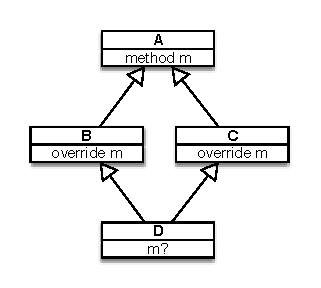
\includegraphics{figures/diamond.eps}
    \subcaption{The diamond problem} \label{fig:diamond}
  \end{subfigure} ~
  \begin{subfigure}[b]{0.45\textwidth}
    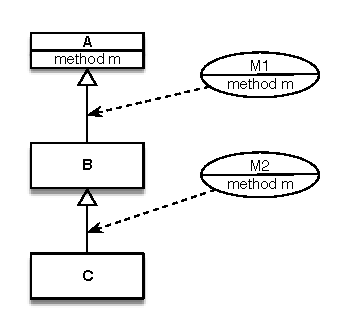
\includegraphics{figures/mixin.eps}
    \subcaption{Mixin composition} \label{fig:mixin}
  \end{subfigure}
  \caption{Multiple inheritance and mixins}
\end{figure}


Mixins and traits are two well-studied mechanisms to provide some form of
multiple inheritance. Mixins~\citep{bracha1990mixin} provide a simple mechanism
for multiple inheritance without the ambiguity issue. A mixin is a subclass
declaration parameterized over a superclass. Or simply put, a mixin can be
treated as a function from classes to classes. Thus the same mixin can be used to
extend a variety of parent classes with the same set of features.
\Cref{fig:mixin} shows a typical class hierarchy when using mixins. In the mixin
model, a class can inherit from another class by means of single inheritance as
usual. Apart from that, it can also have several mixins applied \textit{one at a
  time}. Let us take a close look at \cref{fig:mixin}. Both mixins
\lstinline{M1} and \lstinline{M2} contain a method \lstinline{m}, a question
arises as to which one is inherited in the class \lstinline{C}. The answer is
\lstinline{m} from the mixin \lstinline{M2}. This is because mixin composition
is \textit{linear}: methods defined in mixins appearing later override all the
identically named methods of earlier mixins. While this simple mechanism does
avoid conflicts, it also lead to other problems. For example, though we can
obtain the method \lstinline{m} from the mixin \lstinline{M1} by switching the
order of \lstinline{M1} and \lstinline{M2}, no suitable order of composition
exists to obtain \lstinline{m} from the superclass \lstinline{A}.

In respondence to the problems in the then compositional models,
\citet{scharli2003traits} proposed a mechanism called \textit{traits} as a
better way to foster code reuse in object-oriented programs. A trait is
essentially \textit{a set of pure methods}, divorced from any class hierarchy. A
trait \textit{provides} a set of methods to implement the behavior, and it may
also specify a set of \textit{required methods} that parameterize the provided
behavior. \Cref{fig:trait} shows a simple trait \lstinline{TCircle}, which
provides two methods \lstinline{hash} and \lstinline{area}, and requires a
method \lstinline{radius}. A class is then constructed by inheriting from a
superclass and incorporating a collection of traits, as shown in
\cref{fig:trait:conflict}. Also notice that there is a conflicting method
\lstinline{hash} that is provided by both \lstinline{TCircle} and
\lstinline{TDraw}. This is where the trait model is very different from the
mixin model. Unlike mixins that force a linear order in their composition,
traits can be composed in arbitrary order, and as a consequence, conflicting
methods must be resolved \textit{explicitly}, either by overriding the
conflicting methods, or by excluding a method from all but one trait.
\citet{scharli2003traits} discuss several other issues with mixins, which can be
improved by traits. We refer to their paper for a detailed account of traits.


\begin{figure}
  \centering
  \begin{subfigure}[b]{0.45\textwidth}
    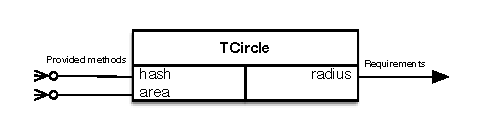
\includegraphics[scale=0.85]{figures/trait1.eps}
    \subcaption{A simple trait} \label{fig:trait}
  \end{subfigure} ~
  \begin{subfigure}[b]{0.45\textwidth}
    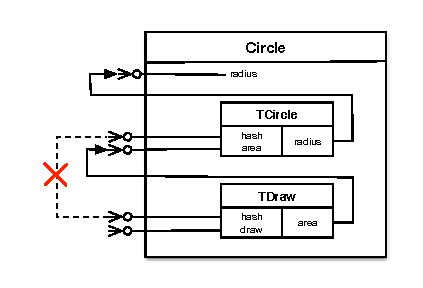
\includegraphics{figures/trait3.eps}
    \subcaption{Trait composition with conflicts} \label{fig:trait:conflict}
  \end{subfigure}
  \caption{Traits and conflicts}
\end{figure}

%%% Local Variables:
%%% mode: latex
%%% TeX-master: "../Thesis"
%%% org-ref-default-bibliography: ../Thesis.bib
%%% End:

  
%%%%%%%%%%%%%%%%%%%%%%%%%%%%%%%%%%%%%%%%%%%%%%%%%%%%%%%%%%%%%%%%%%%%%%%%
\chapter{Semantics of the \namee Calculus}
\label{chap:nested}
%%%%%%%%%%%%%%%%%%%%%%%%%%%%%%%%%%%%%%%%%%%%%%%%%%%%%%%%%%%%%%%%%%%%%%%%

This chapter presents \namee, a calculus with disjoint intersection types that
features both BCD-style subtyping and the merge operator, which we believe
capture the essence of nested composition. We illustrate this by showing a neat
solution to the Expression Problem based on family polymorphism. We then discuss
the algorithmic aspects of \namee. The coherence property of \namee is discussed
in \cref{chap:coherence:simple}.

\section{Introduction}

\namee is a simple calculus with records and disjoint intersection types that
supports \emph{nested composition}. Nested composition enables encoding simple
forms of family polymorphism. More complex forms of family polymorphism,
involving binary methods~\citep{bruce1995binary} and mutable state are not yet
supported, but are interesting avenues for future work. Nevertheless, in \namee,
it is possible, for example, to encode Ernst's elegant family-polymorphism
solution~\citep{Ernst_2001} to the Expression Problem (cf.
\cref{nested:sec:overview}). Compared to \oname the essential novelty of
\namee are distributivity rules between function/record types and intersection
types. These rules are the delta that enable extending the simple forms of
multiple inheritance/composition supported by \oname into a more powerful form
supporting nested composition. The distributivity rule between function types
and intersections is common in calculi with intersection types aimed at
capturing the set of all strongly normalizable terms, and was first proposed by
\citet{Barendregt_1983} (BCD). However the distributivity rule is not common in
calculi or languages with intersection types aimed at programming. For example
the rules employed in languages that support intersection types (such as Scala,
TypeScript, Flow or Ceylon) lack distributivity rules. Moreover distributivity
is also missing from several calculi with a merge operator. This includes all
calculi with disjoint intersection types~\citep{oliveira2016disjoint,
  alpuimdisjoint} and \citeauthor{dunfield2014elaborating}'s work on elaborating
intersection types~\citep{dunfield2014elaborating}, which was the original
foundation for \oname. A possible reason for this omission in the past is that
distributivity adds substantial complexity (both algorithmically and
meta-theoretically), without having any obvious practical applications. This
thesis shows how to deal with the complications of BCD subtyping, while
identifying a major reason to include it in a programming language: BCD enables
nested composition and subtyping, which is of significant practical interest.

%The distributivity rules for records are
%new. Moreover, as far as we know, no previous work
%establishes the relation between BCD-style subtyping and nested composition.

\namee differs significantly from previous BCD-based calculi in that it has to
deal with the possibility of incoherence, introduced by the merge operator. Incoherence
is a non-issue in the previous BCD-based calculi because they do not feature
this merge operator or any other source of incoherence.
Although previous work on disjoint intersection types
proposes a solution to coherence, the solution imposes several ad-hoc restrictions
to guarantee the uniqueness of the elaboration and thus allow for a simple
syntactic proof of coherence (cf. \cref{sec:comparision}). Most
importantly, it makes it hard or impossible to adapt the proof to extensions of
the calculus, such as the new subtyping rules required by the BCD system.

In \namee we remove the brittleness of the previous syntactic method to prove
coherence, by employing a more semantic proof method based on \emph{logical
  relations}~\citep{tait, plotkin1973lambda, statman1985logical}. This new proof method has several
advantages. Firstly, with the new proof method, several restrictions that were
enforced by \oname to enable the syntactic proof method are removed. For example
the work on \oname has to carefully distinguish between so-called \emph{top-like
  types} and other types.
%This is necessary because top-like types can be
%non-disjoint (unlike other types), and yet they need to be allowed in a calculus
%with top types.
In \namee this distinction is not necessary; top-like types are handled like all
other types. Secondly, the method based on logical relations is more powerful
because it is based on semantic rather than syntactic equality. Finally, the
removal of the ad-hoc side-conditions makes adding new extensions, such as
support for BCD-style subtyping, easier. In order to deal with the complexity of
the elaboration semantics of \namee, we employ binary logical relations that are
heterogeneous, parameterized by two types; the fundamental property is also
reformulated to account for bidirectional type-checking.



\section{\namee by Examples}
\label{nested:sec:overview}

This section illustrates \namee with an encoding of a family polymorphism
solution to the expression problem, and informally presents its salient
features.


%-------------------------------------------------------------------------------
\subsection{The Expression Problem, \namee Style}

The \namee calculus allows us to solve the expression problem in a way that is
very similar to \citeauthor{Ernst_2001}'s \textsf{gbeta} solution in \cref{sec:ernst}.
However, the underlying mechanisms of \namee are quite different from those of
\textsf{gbeta}. In particular, \namee features a structural type system in which we can
model objects with records, and object types with record types. For instance, we
model the interface of \lstinline{Lang.Exp} with the singleton record type
\lstinline${ print : String }$. For the sake of conciseness, we use \lstinline{type} aliases
to abbreviate types.
\lstinputlisting[linerange=4-4]{./examples/overview.sl}% APPLY:linerange=PRINT_INTERFACE
Similarly, we capture the interface of the \lstinline{Lang} family in a record,
with one field for each case's constructor.
\lstinputlisting[linerange=8-8]{./examples/overview.sl}% APPLY:linerange=LANG_FAMILY
Here is the implementation of \lstinline{Lang}.
\lstinputlisting[linerange=17-24]{./examples/overview.sl}% APPLY:linerange=LANG_IMPL
We assume several primitive types: fixed width integers \lstinline{Int},
\lstinline{Double} for numeric operations and \lstinline{String} for text
manipulation. A \namee program consists of a collection of definitions and
declarations, separated by semicolon \lstinline{;}.

% - - - - - - - - - - - - - - - - - - - - - - - - - - - - - - - - - - - - - - - -
\paragraph{Adding evaluation.}
We obtain \lstinline{IPrint & IEval}, which is the corresponding type for \lstinline{LangEval.Exp}, by
intersecting \lstinline{IPrint} with \lstinline{IEval} where
\lstinputlisting[linerange=29-29]{./examples/overview.sl}% APPLY:linerange=EVAL_INTERFACE
The type for \lstinline{LangEval} is then
\lstinputlisting[linerange=34-37]{./examples/overview.sl}% APPLY:linerange=EVAL_PRINT_INTERFACE
We obtain an implementation for \lstinline{LangEval} by merging the existing
\lstinline{Lang} implementation \lstinline{implLang} with the new evaluation
functionality \lstinline{implEval} using the merge operator \lstinline{,,}.
\lstinputlisting[linerange=45-53]{./examples/overview.sl}% APPLY:linerange=EVAL_PRINT_IMPL

% - - - - - - - - - - - - - - - - - - - - - - - - - - - - - - - - - - - - - - - -
\paragraph{Adding negation.}
Adding negation to \lstinline{Lang} works similarly.
\lstinputlisting[linerange=57-65]{./examples/overview.sl}% APPLY:linerange=LANG_NEG
% \begin{Verbatim}[xleftmargin=10mm,fontsize=\relscale{.80}]
% type LangNeg = Lang & { neg : IPrint -> IPrint }

% implLangNeg : LangNeg
% implLangNeg = implLang ,, implNeg

% implNeg = { neg = \a.{print = "-" ++ a.print } }
% \end{Verbatim}

% - - - - - - - - - - - - - - - - - - - - - - - - - - - - - - - - - - - - - - - -
\paragraph{Putting everything together.}
Finally, we can combine the two extensions and provide the missing
implementation of evaluation for the negation case.
\lstinputlisting[linerange=70-80]{./examples/overview.sl}% APPLY:linerange=LANG_FINAL
We can test \lstinline{implLangNegEval} by creating an object that represents $-2 + 3$, which is able to print and evaluate at the same time.
\lstinputlisting[linerange=98-100]{./examples/overview.sl}% APPLY:linerange=TEST



%- - - - - - - - - - - - - - - - - - - - - - - - - - - - - - - - - - - - - - - -
\paragraph{Multi-field records.}
Recall that in \cref{bg:sec:intersection}, we show how to model multi-field records by
single-field records. Thus \namee does not have multi-field record types built in.
They are merely syntactic sugar for intersections of single-field record types.
Hence, the following is an equivalent definition of \lstinline{Lang}:
\lstinputlisting[linerange=13-13]{./examples/overview.sl}% APPLY:linerange=LANG_FAMILY2
Similarly, the multi-field record expression in the definition of
\lstinline{implLang} is syntactic sugar for the explicit merge of two
single-field records.
\begin{lstlisting}
implLang : Lang = { lit = ... } ,, { add = ... };
\end{lstlisting}

%- - - - - - - - - - - - - - - - - - - - - - - - - - - - - - - - - - - - - - - -
\paragraph{Subtyping.}
A distinctive difference compared to \textsf{gbeta} is that many more \namee types are related through
subtyping. Indeed, \textsf{gbeta} is unnecessarily conservative~\citep{ernst_hoh}: none of the families is related
through subtyping, nor is any of the class members of one family related to any
of the class members in another family. For instance, \lstinline{LangEval} is
not a subtype of \lstinline{Lang}, nor is \lstinline{LangNeg.Lit} a subtype
of \lstinline{Lang.Lit}.

In contrast, subtyping in \namee is much more nuanced and depends entirely on the
structure of types. The primary source of subtyping are intersection types:
any intersection type is a subtype of its components. For instance, 
\lstinline{IPrint & IEval} is a subtype of both \lstinline{IPrint} and
\lstinline{IEval}. Similarly \lstinline{LangNeg = Lang & NegPrint} is a subtype
of \lstinline{Lang}. Compare this to \textsf{gbeta} where \lstinline{LangEval.Expr} is
not a subtype of \lstinline{Lang.Expr}, nor is the family \lstinline{LangNeg} a
subtype of the family \lstinline{Lang}.

However, \textsf{gbeta} and \namee agree that \lstinline{LangEval} is not a subtype of
\lstinline{Lang}. The \namee-side of this may seem contradictory at first, as we
have seen that intersection types arise from the use of the merge operator.
We have created an implementation for \lstinline{LangEval} with
\lstinline{implLang ,, implEval} where \lstinline{implLang} has type \lstinline{Lang}, which
suggests that \lstinline{LangEval} is a subtype of \lstinline{Lang}.
Yet, there is a flaw in our reasoning:
strictly speaking, \lstinline{implLang ,, implEval} is not of
type \lstinline{LangEval} but instead of type \lstinline{Lang & EvalExt}, where
\lstinline{EvalExt} is the type of \lstinline{implEval}:
\lstinputlisting[linerange=41-41]{./examples/overview.sl}% APPLY:linerange=EVAL_INTERFACE2

Nevertheless, the definition of \lstinline{implLangEval} is valid because
\lstinline{Lang & EvalExt} is a subtype of \lstinline{LangEval}.
Indeed, if we consider for the sake of simplicity only the \lstinline{lit}
field, we have that \lstinline{(Int -> IPrint) & (Int -> IEval)} is a
subtype of \lstinline{Int -> IPrint & IEval}. This follows from a standard
subtyping axiom for distributivity of functions and intersections in the BCD system inherited by \namee.
In conclusion, \lstinline{Lang & EvalExt} is a subtype of both \lstinline{Lang}
and of \lstinline{LangEval}. However, neither of the latter two types is a subtype of the other.
Indeed, \lstinline{LangEval} is not a subtype of \lstinline{Lang} as the type
of \lstinline{add} is not covariantly refined and thus admitting the subtyping
is unsound. For the same reason \lstinline{Lang} is not a subtype of \lstinline{LangEval}.


A summary of the various relationships between the language components is shown
in \cref{fig:diagram}. Admittedly, the figure looks quite complex because our
calculus has a structural type system (as often more foundational calculi
do) where more types are related through subtyping, whereas mainstream object-oriented
languages have nominal type systems.



\begin{figure}[t]
  \centering
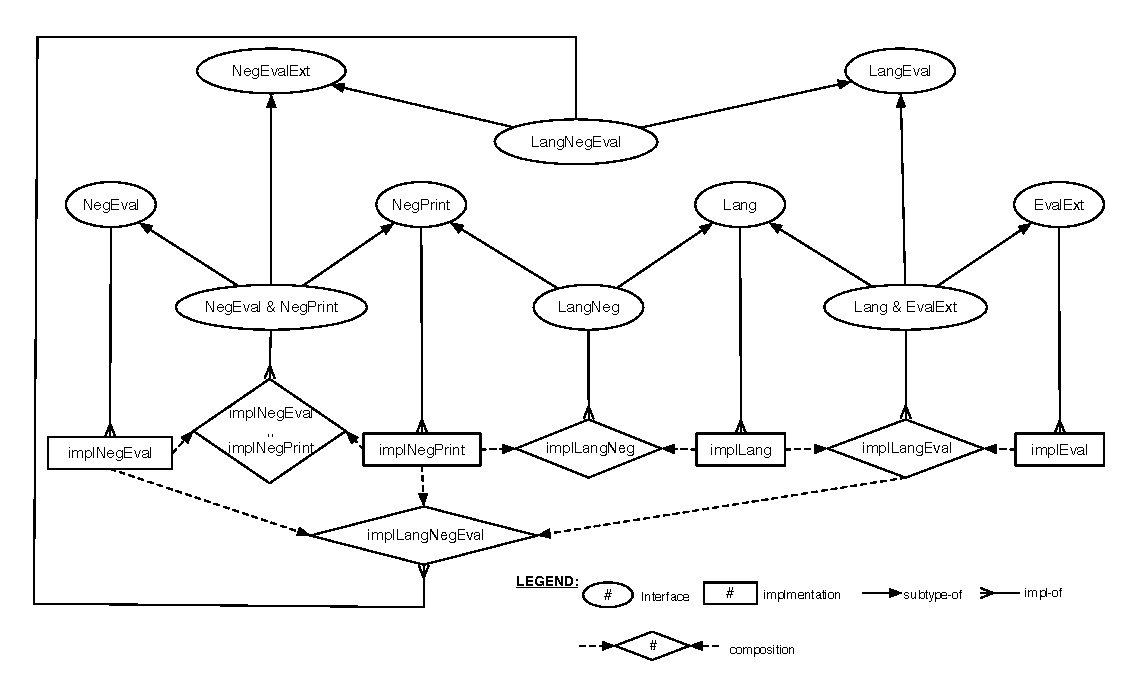
\includegraphics[scale=0.75]{figures/diagram.eps}
\caption{Summary of the relationships between language components}
\label{fig:diagram}
\end{figure}


\paragraph{Stand-alone extensions.}
Unlike in \textsf{gbeta} and other class-based inheritance systems, in \namee
the extension \lstinline{implEval} is not tied to \lstinline{LangEval}. In that
sense, it resembles trait and mixin systems that can apply the same extension
to different classes. However, unlike those systems, \lstinline{implEval} can also
exist as a value on its own, i.e., it is not an extension per se.

%-------------------------------------------------------------------------------
% \subsection{Disjoint Intersection Types and Ambiguity}

% The above example shows that intersection types and the merge operator
% are closely related to multiple
% inheritance. Indeed, they share a major concern with multiple inheritance,
% namely ambiguity. When a subclass inherits an implementation of the same
% method from two different parent classes, it is unclear which of the two
% methods is to be adopted by the subclass. In the case where the two parent classes
% have a common superclass, this is known as the \emph{diamond problem}.
% The ambiguity problem also appears in \namee,
% e.g., if we merge two numbers to obtain $\mer{1}{2}$ of type
% $\inter{\mathsf{Int}}{\mathsf{Int}}$. Is the result of $\mer{1}{2} + 3$
% either $4$ or $5$?

% Disjoint intersection types offer to statically detect potential ambiguity and
% to ask the programmer to explicitly resolve the ambiguity by rejecting the
% program in its ambiguous form. In the previous work on \oname, ambiguity is
% avoided by dictating that all intersection types have to be disjoint, i.e.,
% $\inter{\mathsf{Int}}{\mathsf{Int}}$ is ill-formed because the first component
% has the same type as the second.


% Disjoint intersection types ensure unambiguity and conflicts are
% statically detected and manually resolved by programmers. This
% is similar to the trait model.


% Local Variables:
% TeX-master: "../../Thesis"
% org-ref-default-bibliography: ../../Thesis.bib
% End:


\newcommand{\rulehl}[2][gray!40]{%
  \colorbox{#1}{$\displaystyle#2$}}

\section{Syntax and Semantics}
\label{sec:typesystem}

In this section we formally present the syntax and semantics of \namee. Compared
to prior work~\cite{alpuimdisjoint, oliveira2016disjoint}, \namee has a more
powerful subtyping relation. The new subtyping relation is inspired by BCD-style
subtyping, but with two noteworthy differences: subtyping is coercive (in
contrast to traditional formulations of BCD); and it is extended with records.
We also have a new target language with explicit coercions inspired by the coercion calculus of
Henglein~\cite{Henglein_1994}. A full technical comparison between \namee and \oname can be found in \cref{sec:comparision}.


\subsection{Syntax}

\Cref{fig:source} shows the syntax of \namee.
% with the differences from \oname \hll{highlighted}.
% \namee is a simple calculus with intersection types, the merge operator
% and singleton records.
For brevity of the meta-theoretic study, we do not
consider primitive operations on integers, or other primitive types.
They can be easily added to the language, and our prototype implementation is
indeed equipped with common primitive types and their operations.
Metavariables $[[A]], [[B]], [[C]]$ range over types. Types include the type of integers
$[[nat]]$, a top type $[[Top]]$, function types $[[A -> B]]$, intersection types
$[[A & B]]$, and singleton record types $[[ {l : A} ]]$. Metavariable $[[ee]]$
ranges over expressions. Expressions include variables $[[x]]$, integers $[[i]]$,
a canonical top value $[[Top]]$, lambda abstractions $[[\x . ee]]$,
applications $[[ee1 ee2]]$, merges $[[ee1 ,, ee2]]$, annotated terms $[[ee : A]]$,
singleton records $[[ {l = ee}]]$, and record selections $[[ee.l ]]$.

\begin{figure}[t]
  \centering
\begin{tabular}{llll}\toprule
  Types & $[[A]], [[B]], [[C]]$ & $\Coloneqq$ & $[[nat]] \mid [[Top]] \mid [[A -> B]]  \mid [[A & B]] \mid [[ { l : A } ]]$ \\
  Expressions & $[[ee]]$ & $\Coloneqq$ & $[[x]] \mid [[i]] \mid [[Top]] \mid [[\x . ee]] \mid [[ee1 ee2]] \mid [[ee1 ,, ee2]] \mid [[ee : A]]  $ \\
  & & $\mid$ & $ [[ { l = ee } ]] \mid [[ee.l]] $ \\
  Typing contexts & $[[GG]]$ & $\Coloneqq$ & $[[empty]] \mid [[GG , x : A]]$ \\ \bottomrule
\end{tabular}
  \caption{Syntax of \namee}
  \label{fig:source}
\end{figure}

\subsection{Declarative Subtyping}

\Cref{fig:subtype_decl} presents the subtyping relation. We ignore the
\hll{highlighted} parts, and explain them later in \cref{sec:elaboration}.

\begin{figure}[t]
  \centering
  \drules[S]{$[[A <: B ~~> c]]$}{Declarative subtyping}{refl, trans, top, rcd, arr, andl, andr, and, distArr, topArr, distRcd, topRcd}
  \caption{Declarative specification of subtyping}
  \label{fig:subtype_decl}
\end{figure}

\paragraph{BCD-Style Subtyping.}
The subtyping rules are essentially those of the BCD type
system~\cite{Barendregt_1983}, extended with subtyping for singleton records.
\Rref{S-top,S-rcd} for top types and record types are straightforward.
\Rref{S-arr} for function subtyping is standard. \Rref{S-andl,S-andr,S-and} for
intersection types axiomatize that $[[A & B]]$ is the greatest lower bound of
$[[A]]$ and $[[B]]$. \Rref{S-distArr} is perhaps the most interesting rule.
This, so-called ``distributivity'' rule, describes the interaction between
the subtyping relations for function types and those for intersection types.
Note that the other direction $[[A1 -> A2 & A3 <: (A1 -> A2) & (A1 -> A3)]]$
and the contravariant distribution $[[ (A1 -> A2) & (A3 -> A2) <: A1 & A3 -> A2 ]]$ are both
derivable from the existing subtyping rules, as shown below:
  \begin{footnotesize}
\begin{mathpar}
  \inferrule*[right=\rref*{S-and}]
  {  \inferrule*[right=\rref*{S-arr}]{ [[ A1 <: A1  ]] \\ [[ A2 & A3 <: A2  ]]  }{[[   A1 -> A2 & A3 <: A1 -> A2  ]]} \\
    \inferrule*[right=\rref*{S-arr}]{ [[ A1 <: A1  ]] \\ [[ A2 & A3 <: A3  ]] }{[[ A1 -> A2 & A3 -> A1 -> A3      ]]}  }
  {  [[ A1 -> A2 & A3 <: (A1 -> A2) & (A1 -> A3)  ]]  }
\end{mathpar}
\begin{mathpar}
  \inferrule*[right=\rref*{S-trans}]
  {  \inferrule*[right=\rref*{S-andl}]{ }{[[ (A1 -> A2) & (A3 -> A2) <: A1 -> A2   ]]} \\
    \inferrule*[right=\rref*{S-arr}]{ [[ A1 & A3 <: A1  ]] \\ [[ A2 <: A2  ]] }{[[ A1 -> A2 <: A1 & A3 -> A2  ]]}  }
  {  [[  (A1 -> A2) & (A3 -> A2) <: A1 & A3 -> A2  ]]   }
\end{mathpar}
  \end{footnotesize}
\Rref{S-distRcd}, which is not found in the original BCD system,
prescribes the distribution of records over intersection types. The two
distributivity rules are the key to enable nested composition. The rule
\rref*{S-topArr} is standard in BCD subtyping, and the new
\rref{S-topRcd} plays a similar role for record types.

\paragraph{Non-Algorithmic.}
The subtyping relation in \cref{fig:subtype_decl} is clearly no more than a
specification due to the two subtyping axioms: \rref{S-refl,S-trans}. A sound
and complete algorithmic version is discussed in \cref{sec:alg}. Nevertheless,
for the sake of establishing coherence, the declarative subtyping relation is
sufficient.


\paragraph{Property of Subtyping.}
The subtyping relation is vacuously \textit{reflexive} and \textit{transitive}.



\subsection{Typing of \namee}


\begin{figure}[t]
  \centering
\drules[T]{$[[GG  |- ee => A ~~> e]]$}{Inference}{top, lit, var, app, anno, proj, merge, rcd}
\drules[T]{$[[GG  |- ee <= A ~~> e]]$}{Checking}{abs, sub}
  \caption{Bidirectional type system of \namee}
  \label{fig:type_system}
\end{figure}

% no gray anymore after this point
\renewcommand{\rulehl}[1]{#1}



The bidirectional type system for \namee is shown in \cref{fig:type_system}.
Again we ignore the \hll{highlighted} parts for now.

% The main difference to \oname is the absence of a well-formedness
% judgement. Unlike \oname, which requires a well-formedness judgement to ensure
% that all intersection types are disjoint, \namee only requires a disjointness
% check at the merge operator. Non-disjoint types such as $[[nat & nat]]$ are
% allowed in other parts of the program.

\begin{comment}
Unlike the development of \oname, which first presents a type assignment
specification, \Cref{fig:type_system} directly present the bidirectional type
system of \namee.
Unfortunately, we found that their declarative type
system is incoherent in nature (even with all the syntactic restrictions).
\jeremy{perhaps add a counter example somewhere?} Again, the reader is advised
to continue ignoring the gray-shaded parts until \cref{sec:elaboration}.
\tom{The above story is a bit confusing to me. Is it the case that the
     \oname paper already was aware of the coherence problem with its
     declarative type system and for that reason (and inference) presented
     a bidirection type system as well? If so, that's not clear.} \jeremy{I
     remember at one point Bruno and I believed the declarative system is
     coherent, it's just hard to prove. Then I found a counterexample. That was
     after \tname paper.  }
\end{comment}


\begin{figure}[t]
  \centering
  \drules[D]{$[[A ** B]]$}{Disjointness}{topL, topR, arr, andL, andR, rcdEq, rcdNeq,ax}
  \drules[Dax]{$[[A **a B]]$}{Disjointness axioms}{sym, intArr, intRcd,arrRcd}
  \caption{Disjointness}
  \label{fig:disjoint}
\end{figure}


\paragraph{Typing Rules and Disjointness.}

As with traditional bidirectional type systems, we employ two modes: the
inference mode ($[[=>]]$) and the checking mode ($[[<=]]$). The inference
judgement $[[GG |- ee => A]]$ says that we can synthesize a type $[[A]]$ for
expression $[[ee]]$ in the context $[[GG]]$. The checking judgement $[[GG |- ee
<= A]]$ checks $[[ee]]$ against $[[A]]$ in the context $[[GG]]$. The
disjointness judgement $[[A ** B]]$ used in \rref{T-merge} is shown in
\cref{fig:disjoint}, which states that the types $[[A]]$ and $[[B]]$ are
\textit{disjoint}. The intuition of two types being disjoint is
that their least upper bound is (isomorphic to) $[[Top]]$. The disjointness judgement is
important in order to rule out ambiguous expressions such as $\mer{1}{2}$. Most
of the typing and disjointness rules are standard and are explained in detail in
previous work~\cite{oliveira2016disjoint, alpuimdisjoint}.
%We refer
%the reader to their papers for further explanation.


\subsection{Elaboration Semantics}
\label{sec:elaboration}

\begin{figure}[t]
  \centering
\begin{tabular}{llll} \toprule
  Types & $[[T]]$ & $\Coloneqq$ & $[[nat]] \mid [[Unit]] \mid [[T1 * T2]] \mid [[T1 -> T2]] $ \\
  Terms & $[[e]]$ & $\Coloneqq$ & $[[x]] \mid [[i]] \mid [[unit]] \mid [[\x . e]] \mid [[e1 e2]] \mid [[<e1, e2>]] \mid [[c e]]$ \\
  Coercions & $[[c]]$ & $\Coloneqq$ & $ [[id]] \mid [[c1 o c2]] \mid [[top]] \mid [[c1 -> c2]] \mid [[<c1, c2>]] \mid [[pp1]] \mid [[pp2]] $ \\
  &  &  $\mid$ & $   [[distArr]] \mid [[topArr]]  $ \\
  Values & $[[v]]$ & $\Coloneqq$ & $[[unit]] \mid [[i]] \mid [[\x.e]] \mid  [[<v1, v2>]] \mid [[(c1 -> c2) v]] \mid [[distArr v]] \mid [[topArr v]] $ \\
  Typing contexts & $[[gg]]$ & $\Coloneqq$ & $[[empty]] \mid [[gg , x : T]]$ \\
  Evaluation Contexts & $[[EE]]$ & $\Coloneqq$ &  $  [[__]] \mid [[EE e]] \mid [[v EE]] \mid [[ < EE , e >  ]] \mid [[ < v , EE > ]] \mid [[ c EE  ]]$ \\ \bottomrule
\end{tabular}
  \caption{\tname syntax}
  \label{fig:target}
\end{figure}

The operational semantics of \namee is given by elaborating source expressions
$[[ee]]$ into target terms $[[e]]$. Our target language \tname is the standard
simply-typed call-by-value $\lambda$-calculus extended with products and coercions.
The syntax of \tname is shown in \cref{fig:target}. The
meta-function $| \cdot |$ shown in \cref{def:type:translate} transforms \namee
types to \tname types, and extends naturally to typing contexts.

\begin{definition}[Type translation from \namee to \tname] \label{def:type:translate}
  \begin{align*}
    | [[nat]] | &= [[nat]] \\
    | [[Top]] | &= \langle \rangle \\
    | [[A -> B]]  | &= [[ | A | -> | B |  ]] \\
    | [[ A & B  ]] | &= [[ | A | * | B |  ]] \\
    | \recordType{l}{A} | &= | A |
  \end{align*}
\end{definition}



\paragraph{Explicit Coercions and Coercive Subtyping.}

The separate syntactic category for explicit coercions is a distinct
difference from the prior works (in which they are regular terms). Our coercions
are based on those of Henglein~\cite{Henglein_1994}, and we add more forms due to our
extra subtyping rules.
Metavariable $[[c]]$ ranges over coercions.\footnote{Coercions $[[pp1]]$ and $[[pp2]]$ subsume the first and second projection of pairs, respectively.}
Coercions express the conversion
of a term from one type to another. Because of the addition of coercions, the
grammar contains explicit coercion applications $[[c e]]$ as a term, and various
unsaturated coercion applications as values. The use of explicit coercions is useful for the new semantic
proof of coherence based on logical relations.
The subtyping judgement in \cref{fig:subtype_decl} has the form $[[A <: B ~~> c]]$, which says that the
subtyping derivation of $[[A <: B]]$ produces a coercion $[[c]]$ that converts
terms of type $[[ |A| ]]$ to type $[[ |B| ]]$. Each subtyping rule has its own
specific form of coercion.

%The meaning of the different forms of coercions becomes clear in \tom{Section
%  TODO} \jeremy{it's a paragraph, how to refer it?} which explains coercive
%subtyping.\bruno{Why not discuss the form of coercions directly here?}


\paragraph{Target Typing.}
The typing of \tname has the form $[[gg |- e : T]]$, which is entirely standard. Only the typing of coercion
applications, shown below, deserves attention:
\begin{mathpar}
\drule{t-capp}
\end{mathpar}
Here the judgement $[[c |- T1 tri T2]]$ expresses the typing of coercions, which
are essentially functions from $[[T1]]$ to $[[T2]]$. Their typing
rules correspond exactly to the subtyping rules of \namee, as
shown in \cref{fig:co}.

\begin{figure}[t]
  \centering
  \drules[ct]{$[[c |- T1 tri T2]]$}{Coercion typing}{refl, trans, top, topArr, arr, pair, projl, projr, distArr}
  \caption{Coercion typing}
  \label{fig:co}
\end{figure}

\paragraph{Dynamic Semantics.}

\begin{figure}[t]
  \centering
\drules[r]{$[[e --> e']]$}{Single-step reduction}{id, trans, top, topArr, pair, arr, distArr, projl, projr, app, ctxt}
  \caption{Dynamic semantics of \tname}
  \label{fig:coercion_red}
\end{figure}

The dynamic semantics of \tname is shown in \cref{fig:coercion_red}. We write
$[[e --> e']]$ for reduction of expressions. The first three lines are reduction
rules for coercions. They do not contribute to computation but merely rearrange
coercions. Our coercion reduction rules are quite standard but not efficient in
terms of space. Nevertheless, there is existing work on space-efficient
coercions~\cite{Siek_2015, herman2010space}, which should be applicable to our
work as well. \Rref{r-app} is the usual $\beta$-rule that performs actual
computation, and \rref{r-ctxt} handles reduction under an evaluation context. As
standard, $[[-->>]]$ is the reflexive, transitive closure of $[[-->]]$.
Now we can show that \tname is type safe:
\begin{theorem}[Preservation]
  If $[[empty |- e : T]]$ and $[[e --> e']]$, then $[[empty |- e' : T]]$.
\end{theorem}
\begin{theorem}[Progress]
  If $[[empty |- e : T]]$, then either $[[e]]$ is a value, or there exists $[[e']]$ such
  that $[[e --> e']]$.
\end{theorem}




\paragraph{Elaboration.}
\begin{comment}
The subtyping judgement in \cref{fig:subtype_decl} has the form $[[A <: B ~~> c]]$, which says that the subtyping
derivation of $[[A <: B]]$ produces a coercion $[[c]]$ that is used to convert a
term of type $[[ |A| ]]$ to type $[[ |B| ]]$. Each
subtyping rule has its own specific form of coercion.
\end{comment}
We are now in a position to explain the elaboration judgements $[[GG |- ee
=> A ~~> e]]$ and $[[GG |- ee <= A ~~> e]]$ in \cref{fig:type_system}. The only
interesting rule is \rref{T-sub}, which applies the coercion $[[c]]$ produced by
subtyping to the target term $[[e]]$ to form a coercion application
$[[c e]]$. All the other rules do straightforward translations between
source and target expressions.


To conclude, we show two lemmas that relate \namee expressions
to \tname terms.
% (Note that in this and subsequent sections, we only provide
% a proof sketch for each lemma and theorem. We refer the interested reader
% to our Coq development for the full proofs.)

\begin{lemma}[Coercions preserve types]
  If $[[A <: B ~~> c]]$, then $[[c |-  |A| tri |B|]]$.
  \label{lemma:sub-correct}
\end{lemma}
\begin{proof}
  By structural induction on the derivation of subtyping.
\end{proof}


\begin{lemma}[Elaboration soundness] We have that:
  \begin{itemize}
  \item If $[[GG |- ee => A ~~> e]]$, then $|\Gamma| \vdash e : |A| $.
  \item If $[[GG |- ee <= A ~~> e]]$, then $|\Gamma| \vdash e : |A| $.
  \end{itemize}
\end{lemma}
\begin{proof}
  By structural induction on the derivation of typing.
\end{proof}

\subsection{Comparison with \oname}
\label{sec:comparision}

Below we identify major differences between \namee and \oname, which, when
taken together, yield a simpler and more elegant system. The differences may seem
superficial, but they have far-reaching impacts on the semantics, especially on
coherence, our major topic in \cref{chap:coherence:simple}.

\paragraph{No Ordinary Types.}

Apart from the extra subtyping rules, there is an important difference from the
\oname subtyping relation. The subtyping relation of \oname employs an
auxiliary unary relation called $\mathsf{ordinary}$, which plays a fundamental
role for ensuring coherence and obtaining an
algorithm~\cite{Davies_2000}. The \namee calculus discards the notion of
ordinary types completely; this yields a clean and elegant formulation of the
subtyping relation. Another minor difference is that due to the addition of the
transitivity axiom (\rref{S-trans}), \rref{S-andl,S-andr} are simplified: an
intersection type $[[A & B]]$ is a subtype of both $[[A]]$ and $[[B]]$, instead
of the more general form $[[ A & B <: C]]$.

% \paragraph{Example}
% The following example shows the derivation tree of the subtyping example
% presented in \cref{sec:overview}. \jeremy{A derivation of the nested composition
%   example? }


\paragraph{No Top-Like Types.}

There is a notable difference from the coercive subtyping of \oname. Because of
their syntactic proof method, they have special treatment for coercions of
\textit{top-like types} in order to retain coherence. For \namee, as
with ordinary types, we do not need this kind of ad-hoc treatment, thanks to the
adoption of a more powerful proof method (cf. \cref{chap:coherence:simple}).




\paragraph{No Well-Formedness Judgement.}

A key difference from the type system of \oname is the complete omission of the
well-formedness judgement. In \oname, the well-formedness judgement $[[GG |- A]]$
appears in both \rref{T-abs,T-sub}. The sole purpose of this judgement is
to enforce the invariant that all intersection types are disjoint. However, as
\cref{chap:coherence:simple} will explain, the syntactic restriction is unnecessary for
coherence, and merely complicates the type system. The \namee calculus discards
this well-formedness judgement altogether in favour of a simpler design that is
still coherent. An important implication is that even without adding BCD subtyping,
\namee is already more expressive than \oname: an expression such as $1 : [[nat & nat]]$ is accepted in
\namee but rejected in \oname. This simplification is based on an important
observation: incoherence can only originate in merges. Therefore disjointness
checking is only necessary in \rref{T-merge}.


% Local Variables:
% TeX-master: "../../Thesis"
% org-ref-default-bibliography: ../../Thesis.bib
% End:


\section{Algorithmic Subtyping}
\label{sec:alg}

This section presents an algorithm that implements the subtyping relation in
\cref{fig:subtype_decl}. While BCD subtyping is well-known, the
presence of a transitivity axiom in the rules means that the system is
not algorithmic. This raises an obvious question: how to obtain an
algorithm for this subtyping relation? Laurent~\cite{Laurent12note} has shown that simply dropping
the transitivity rule from the BCD system is not possible without losing expressivity. Hence, this avenue for
obtaining an algorithm is not available. 
%Moreover, even if transitivity elimination
%would be possible, the remaining rules are still highly overlapping, and pose
%difficulties for an implementation.  
Instead, we adapt Pierce's decision
procedure~\cite{pierce1989decision} for a subtyping system (closely
related to BCD) to obtain a sound and complete algorithm for our
BCD extension. Our algorithm extends Pierce's decision
procedure with subtyping of singleton records and
coercion generation. We prove in Coq that the algorithm is sound and complete with
respect to the declarative version. At the same time we
find some errors and missing lemmas in Pierce's original manual proofs.

%The algorithm is implemented in our
%prototype implementation. \jeremy{should i say more about implementation?}

%See \cref{sec:alg} for the details. 
%\bruno{The meaning of the paragraph is somewhat obscure to me. After
%  discussing with Tom, it seems that what may be meant here is that we
%cannot do cut elimination, which is a common process that you can try
%for certain systems with subtyping. However Pierce managed to find
%another way to get a sound/complete algorithmic system. Maybe 
%the text can be improved.}


\subsection{The Subtyping Algorithm}

\begin{figure}[t]
  \centering
  \begin{small}
  \drules[A]{$[[fs |- A <: B ~~> c]]$}{Algorithmic subtyping}{and, arr, rcd, top, arrNat, rcdNat, andNOne, andNTwo, nat}
  \end{small}
  \caption{Algorithmic subtyping of \name}
  \label{fig:algorithm}
\end{figure}


\Cref{fig:algorithm} shows the algorithmic subtyping judgement $[[fs |- A <: B ~~> c]]$.
This judgement is the algorithmic counterpart of the declarative
judgement $[[A <: fs -> B ~~> c]]$, where the symbol $[[fs]]$ stands for a
queue of types and labels. Definition~\ref{def:fs} converts a queue to a type:
\begin{definition} $[[fs -> A]]$ is inductively defined as follows: \label{def:fs}
  \begin{mathpar}
    [[ [] -> A]] = [[A]] \and
    [[ (fs , B) -> A]] = [[fs -> (B -> A)]] \and
    [[ (fs , {l}) -> A]] = [[fs -> {l : A}]]
  \end{mathpar}
\end{definition}
For instance, if $[[fs]] = [[A]] , [[B]] , \{[[l]]\} $, then $[[fs -> C]]$ abbreviates $ [[A -> B -> {l : C}]]$.

The basic idea of $[[fs |- A <: B ~~> c]]$ is to first perform a structural
analysis of $[[B]]$, which descends into both sides of $[[&]]$'s (\rref{A-and}),
into the right side of $[[->]]$'s (\rref{A-arr}), and into the fields of records
(\rref{A-rcd}) until it reaches one of the two base cases, $[[nat]]$ or
$[[Top]]$. If the base case is $[[Top]]$, then the subtyping holds trivially
(\rref{A-top}). If the base case is $[[nat]]$, the algorithm performs a
structural analysis of $[[A]]$, in which $[[fs]]$ plays an important role. The
left sides of $[[->]]$'s are pushed onto $[[fs]]$ as they are encountered in
$[[B]]$ and popped off again later, left to right, as $[[->]]$'s are encountered
in $[[A]]$ (\rref{A-arrNat}). Similarly, the labels are pushed onto $[[fs]]$ as
they are encountered in $[[B]]$ and popped off again later, left to right, as
records are encountered in $[[A]]$ (\rref{A-rcdNat}). The remaining rules are
similar to their declarative counterparts. Let us illustrate the algorithm
with an example
derivation (for space reasons we use $[[N]]$ and $[[S]]$ to denote $[[nat]]$ and $[[string]]$ respectively),
which is essentially the one used by the \lstinline{add} field in \cref{sec:overview}. The
readers can try to give a corresponding derivation using the declarative
subtyping and see how \rref{S-trans} plays an essential role there.
\begin{small}
\begin{mathpar}
  \inferrule*[right=\rref*{A-rcd}]
  { \inferrule*[right=\rref*{A-arr}(\textit{twice})]
    { \inferrule*[right=\rref*{A-and}]
      { D \\ D' }
      { \{ [[l]]  \}, [[N & S]] ,[[N & S]] \vdash [[{l : N -> N -> N} & {l : S -> S -> S} ]] \prec : [[N & S]] }  }
    { \{ [[l]]  \} \vdash [[{l : N -> N -> N} & {l : S -> S -> S} ]] \prec : [[ N & S -> N & S -> N & S ]]}      }
  {  [[{l : N -> N -> N} & {l : S -> S -> S}]] \prec : [[{l : N & S -> N & S -> N & S}]]   }
\end{mathpar}
\end{small}
where the sub-derivation $D$ is shown below ($D'$ is similar):
\begin{small}
\begin{mathpar}
\inferrule*[right=\rref*{A-andN1}]
        { \inferrule*[right=\rref*{A-rcdNat}]
          { \inferrule*[right=\rref*{A-arrNat}]
            { \inferrule*{ \dots } { [[N & S]] \prec : [[N]] }
              \\
              \inferrule* {\dots} { [[N & S]] \vdash [[N -> N]] \prec : [[N]] }     }
            {[[N & S]] ,[[N & S]] \vdash [[N -> N -> N]] \prec : [[N]]} }
          { \{ [[l]]  \}, [[N & S]] ,[[N & S]] \vdash [[{l : N -> N -> N}]] \prec : [[N]] } }
        { \{ [[l]]  \}, [[N & S]] ,[[N & S]] \vdash [[{l : N -> N -> N} & {l : S -> S -> S} ]] \prec : [[N]] }
\end{mathpar}
\end{small}
Now consider the coercions. Algorithmic subtyping uses the same set of
coercions as declarative subtyping. However, because algorithmic
subtyping has a different structure, the rules generate slightly more
complicated coercions. Two meta-functions $\llbracket \cdot \rrbracket_{\top}$
and $\llbracket \cdot \rrbracket_{\&}$ used in \rref{A-top,A-and} respectively,
are meant to generate correct forms of coercions. They are defined recursively
on $[[fs]]$ and are shown in \cref{fig:coercion}.

\begin{figure}[t]
    \centering
    \begin{small}
    \begin{subfigure}[b]{0.5\textwidth}
      \begin{align*}
        [[ < [] >1 ]] &=  [[top]] \\
        [[ < { l } , fs >1 ]] &= [[ {l : < fs >1} o < l >  ]] \\
        [[ < A , fs >1 ]] &= [[(top -> < fs >1) o (topArr o top)]]
      \end{align*}
    \end{subfigure} ~
    \begin{subfigure}[b]{0.45\textwidth}
      \begin{align*}
        [[ < [] >2 ]] &=  [[id]] \\
        [[ < { l } , fs >2 ]] &= [[ {l : < fs >2} o distRcd l  ]] \\
        [[ < A , fs >2 ]] &= [[(id -> < fs >2) o distArr]]
      \end{align*}
    \end{subfigure}
    \end{small}
    \caption{Meta-functions of coercions}\label{fig:coercion}
\end{figure}

\subsection{Correctness of the Algorithm}

To establish the correctness of the algorithm, we must show that the algorithm
is both sound and complete with respect to the declarative specification. While
soundness follows quite easily, completeness is much harder. The proof of
completeness essentially follows that of Pierce~\cite{pierce1989decision}
%%\footnote{
%%While transferring \cite{pierce1989decision}'s manual proofs to Coq,
%%we discovered several errors, which will be reported along the way.}
in that we
need to show the algorithmic subtyping is reflexive and
transitive. 


\paragraph{Soundness of the Algorithm.}

The following two lemmas connect the declarative subtyping with the meta-functions.

\begin{lemma} \label{lemma:top}
  $[[ Top <: fs -> Top ~~> < fs >1]]$
\end{lemma}
\begin{proof}
  By induction on the length of $[[fs]]$.
\end{proof}

\begin{lemma} \label{lemma:and}
  $[[(fs -> A) & (fs -> B) <: fs -> (A & B) ~~> < fs >2]]$
\end{lemma}
\begin{proof}
  By induction on the length of $[[fs]]$.
\end{proof}

The proof of soundness is straightforward.
\begin{theorem}[Soundness] \label{thm:soundness}
  If $[[ fs |- A <: B ~~> c]]$ then $[[A]] <: [[fs]] \rightarrow [[B]] [[~~>]] [[c]]$.
\end{theorem}
\begin{proof}
  By induction on the derivation of the algorithmic subtyping and applying \cref{lemma:top,lemma:and} where appropriate.
\end{proof}


\paragraph{Completeness of the Algorithm.}


\newcommand{\UU}[1]{\mathcal{U}(#1)}

Completeness, however, is much harder. The reason is that, due to the use of
$[[fs]]$, reflexivity and transitivity are not entirely obvious. We need to
strengthen the induction hypothesis by introducing the notion of a set,
$\UU{[[A]]}$, of ``reflexive supertypes'' of $[[A]]$, as defined below:
\begin{mathpar}
  \UU{[[Top]]} \defeq \{ [[Top]]  \} \and
  \UU{[[nat]]} \defeq \{ [[nat]]  \} \and
  \UU{[[{l : A}]]} \defeq \{ [[{l : B}]] \mid [[B]] \in \UU{[[A]]}  \} \and
  \UU{[[A & B]]} \defeq \UU{[[A]]} \cup \UU{[[B]]} \cup \{ [[A & B]] \} \and
  \UU{[[A -> B]]} \defeq \{ [[A -> C]] \mid [[C]] \in \UU{[[B]]} \}
\end{mathpar}
We show two lemmas about $\UU{[[A]]}$ that are crucial in the subsequent proofs.
\begin{lemma} \label{lemma:set_refl}
  $[[A]] \in \UU{[[A]]}$
\end{lemma}
\begin{proof}
  By induction on the structure of $[[A]]$.
\end{proof}

\begin{lemma} \label{lemma:set_trans}
  If $[[A]] \in \UU{[[B]]}$ and $[[B]] \in \UU{[[C]]}$, then $[[A]] \in \UU{[[C]]}$.
\end{lemma}
\begin{proof}
  By induction on the structure of $[[B]]$.
\end{proof}

\begin{remark}
  Lemma~\ref{lemma:set_trans} is not found in Pierce's proofs~\cite{pierce1989decision}, which is
  crucial in Lemma~\ref{lemma:refl0}, from which reflexivity (Lemma~\ref{lemma:refl})
  follows immediately.
\end{remark}

% Next we show the following lemma from which reflexivity (Lemma~\ref{lemma:refl})

\begin{lemma} \label{lemma:refl0}
  If $[[fs -> B]] \in \UU{[[A]]}$ then there exists $[[c]]$ such that $[[fs |- A <: B ~~> c]]$.
\end{lemma}
\begin{proof}
  By induction on $\mathsf{size}([[A]]) + \mathsf{size}([[B]]) + \mathsf{size}([[fs]])$.
\end{proof}
% \begin{remark}
%   \cite{pierce1989decision}'s proof is wrong in one case~\cite[pp.~10, Case~ii]{pierce1989decision} because we need \cref{lemma:set_trans} to be able
%   to apply the inductive hypothesis.
% \end{remark}

Now it immediately follows that the algorithmic subtyping is reflexive.

\begin{lemma}[Reflexivity] \label{lemma:refl}
  For every $[[A]]$ there exists $[[c]]$ such that $[[ [] |- A <: A ~~> c]]$.
\end{lemma}
\begin{proof}
  Immediate from Lemma~\ref{lemma:set_refl} and Lemma~\ref{lemma:refl0}.
\end{proof}

We omit the details of the proof of transitivity.
%The proof of transitivity is, to quote \cite{pierce1989decision}, typically
%``the hardest single piece'' of metatheory. We omit the details here for lack of space and
%refer the interested reader to our Coq development.

\begin{lemma}[Transitivity] \label{lemma:trans}
  If $[[ [] |- A1 <: A2 ~~> c1]]$ and $[[ [] |- A2 <: A3 ~~> c2]]$, then there
  exists $[[c]]$ such that $[[ [] |- A1 <: A3 ~~> c]]$.
\end{lemma}

With reflexivity and transitivity in position, we show the main theorem.

\begin{theorem}[Completeness] \label{thm:complete}
  If $[[A <: B ~~> c]]$ then there exists $[[c']]$ such that $[[ [] |- A <: B ~~> c']]$.
\end{theorem}
\begin{proof}
  By induction on the derivation of the declarative subtyping and applying \cref{lemma:refl,lemma:trans} where appropriate.
\end{proof}
\begin{remark}
  Pierce's proof is wrong~\cite[pp.~20, Case~F]{pierce1989decision} in the case
  \begin{mathpar}
  \drule{S-arr}
  \end{mathpar}
  where he concludes from the inductive
  hypotheses $[[ [] |- B1 <: A1]]$ and $[[ [] |- A2 <: B2]]$ that $[[ [] |- A1 -> A2 <: B1 -> B2]]$ (rules 6a and 3).
  However his rule 6a (our \rref{A-arrNat}) only works for \textit{primitive types}, and is thus not applicable in this case. Instead we
  need a few technical lemmas to support the argument.
\end{remark}

\begin{remark}
  It is worth pointing out that the two coercions $[[c]]$ and $[[c']]$ in
  Theorem~\ref{thm:complete} are contextually equivalent, which follows from
  Theorem~\ref{thm:soundness} and Corollary~\ref{lemma:coercion_same}.
\end{remark}

% Local Variables:
% org-ref-default-bibliography: ../paper.bib
% End:

% 
\section{Conclusions and Future Work}
\label{sec:conclusion}

We have proposed \name, a type-safe and coherent calculus with disjoint
intersection types, and support for nested composition/subtyping. \name
improves upon earlier work with a more
flexible notion of disjoint intersection types, which leads to
a clean and elegant formulation of the type system. Due to the added
flexibility we have had to employ a more powerful proof method based on logical
relations to rigorously prove coherence.
We also show how \name supports essential features of family
polymorphism, such as nested composition. We believe \name provides insights into family polymorphism, and
has potential for practical applications for extensible software designs.

A natural direction for future work is to enrich \name with parametric
polymorphism. There is abundant literature on logical relations for parametric
polymorphism~\cite{reynolds1983types} and we foresee no fundamental difficulties
in extending our proof method.\footnote{ Our prototype implementation already
  supports polymorphism, but we are still in the process of extending our Coq
  development with polymorphism.} The main challenge in the definition of the
logical relation is the clause for type variables with arbitrary types. Careful
measures are to be taken to avoid the potential circularity due to
impredicativity. With the combination of parametric polymorphism and nested
composition, an interesting application that we intend to investigate is native
support for a highly modular form of \textit{Object Algebras}~\cite{oliveira2012extensibility, xuan_traits} and \textsc{Visitor}s
(or the finally tagless approach~\cite{CARETTE_2009}).

Another direction for future work is to add mutable references, which would
touch two places in our metatheory: type safety and coherence. For type safety,
we expect that lessons learned from previous work on family polymorphism and
mutability on OO to apply to our work. For example, it is well-known that
subtyping in the presence of mutable state often needs restrictions. Given such
suitable restrictions we expect that type-safety in the presence of mutability
still works. For coherence, it would be a major technical challenge to adjust
our coherence proof and its Coq mechanisation. Logical relations that account
for mutable state (e.g., see Ahmed's thesis~\cite{ahmed2004semantics}) introduce significant complexity.





% For example, we can
% define the object algebra interfaces for the Expression Problem example in
% \cref{sec:overview} as follows:
% \lstinputlisting[linerange=77-78]{../../impl/examples/overview.sl}% APPLY:linerange=LANG_EXT_INTER
% By instantiating \lstinline{E} with \lstinline{IPrint}, i.e.,
% \lstinline{ExpAlg[IPrint]}, we get the interface of the \lstinline{Lang} family.
% In that sense, object algebra interfaces can be viewed as family interfaces.
% Moreover, combining algebras implementing \lstinline{ExpAlg[IPrint]} and
% \lstinline{ExpAlg[IEval]} to form \lstinline{ExpAlg[IPrint & IEval]} is trivial
% with nested composition. Polymorphism also improves code reuse across expressions in the
% base and extended languages. For example, the following creates two expressions,
% one in the base language, the other in the extended language:
% \lstinputlisting[linerange=83-84]{../../impl/examples/overview.sl}% APPLY:linerange=LANG_EXT
% Notice how we can  reuse \lstinline{e1} of the base language in the definition
% of \lstinline{e2}.



% \jeremy{creating expressions using base and extended expressions, and show more reuse}

% \jeremy{future work} \jeremy{mention in passing this rule is unsound with
%   effects, see ``Intersection types and computational effects''}

% Local Variables:
% mode: latex
% TeX-master: "../paper"
% org-ref-default-bibliography: ../paper.bib
% End:




%%% Local Variables:
%%% mode: latex
%%% TeX-master: "../Thesis"
%%% End:


% This ensures that the subsequent sections are being included as root
% items in the bookmark structure of your PDF reader.
\bookmarksetup{startatroot}
\backmatter

  \begingroup
    \let\clearpage\relax
    \glsaddall
    \printglossary[type=\acronymtype]
    \newpage
    \printglossary
  \endgroup

  \printindex
  \printbibliography

\end{document}
